\documentclass[aspectratio=169,11pt]{beamer}

\usetheme{metropolis}

\usepackage[T1]{fontenc}
\usepackage{lmodern}
\usepackage{amsmath,amssymb,bm}
\usepackage{booktabs}
\usepackage{algpseudocode}
\usepackage{array}
\usepackage{tikz}
\usetikzlibrary{positioning,shapes.geometric,arrows.meta,calc,fit,backgrounds,shadows}
\usepackage{pgfplots}
\pgfplotsset{compat=1.18}
\usepgfplotslibrary{groupplots}
\usepackage{xcolor}
\definecolor{ForestGreen}{RGB}{34,110,60}

\graphicspath{{../latex_assets/}{latex_assets/}{./latex_assets/}}

\definecolor{HildesheimRed}{RGB}{51,63,156}
\definecolor{PrismBlue}{RGB}{27,94,99}
\definecolor{PrismGreen}{RGB}{46,125,50}
\definecolor{PrismOrange}{RGB}{179,73,31}
\definecolor{PrismRed}{RGB}{51,63,156}
\definecolor{PrismGray}{RGB}{90,90,90}
\definecolor{PrismLightBlue}{RGB}{228,230,247}
\definecolor{PrismLightGreen}{RGB}{232,245,233}
\definecolor{PrismLightOrange}{RGB}{247,229,219}

\metroset{block=fill, progressbar=frametitle, numbering=fraction, sectionpage=progressbar}
\setbeamercolor{palette primary}{bg=HildesheimRed, fg=white}
\setbeamercolor{frametitle}{bg=HildesheimRed, fg=white}
\setbeamercolor{progress bar}{fg=HildesheimRed, bg=PrismGray!25}
\setbeamercolor{alerted text}{fg=HildesheimRed}
\setbeamercolor{block title alerted}{bg=HildesheimRed!85!black, fg=white}
\setbeamercolor{block body alerted}{bg=HildesheimRed!8, fg=black}
\setbeamercolor{block title}{bg=PrismGray!85!black, fg=white}
\setbeamercolor{block body}{bg=PrismGray!8, fg=black}
\setbeamertemplate{navigation symbols}{}
\setbeamerfont{title}{series=\bfseries}

\newcommand{\metric}[2]{\begin{tabular}{c}\textbf{\Large #1}\\[-1mm]{\scriptsize #2}\end{tabular}}
\newcommand{\yes}{\textcolor{PrismGreen}{\textbf{Yes}}}
\newcommand{\partly}{\textcolor{PrismOrange}{\textbf{Partial}}}
\newcommand{\evidence}[1]{\textcolor{HildesheimRed}{\textbf{#1}}}

\title[Advisor Meeting]{Where the Thesis Stands}
\subtitle{\normalsize How it works, what the experiments show, where it succeeds and where it fails}
\author{Brhanu Atsbaha}
\institute{Universität Hildesheim\\[0.15cm]\small \textbf{Advisors:} Prof. Dr. Thomas Mandl \& Shereen Elsayed}
\date{Advisor meeting --- Monday 14 September 2026}


\newcommand{\works}{\textcolor{PrismGreen}{\textbf{Works}}}
\newcommand{\fails}{\textcolor{PrismOrange}{\textbf{Fails}}}
\newcommand{\thin}{\textcolor{HildesheimRed}{\textbf{Thin}}}
\setbeamercolor{block title example}{bg=PrismGreen!80!black, fg=white}
\setbeamercolor{block body example}{bg=PrismLightGreen, fg=black}

\begin{document}

\maketitle

\begin{frame}{Starting From What You Already Read}
\normalsize
The draft and slides I sent already carried the retraction. You have both read:
\vspace{2mm}
\begin{itemize}\small
  \setlength\itemsep{1mm}
  \item that a plain confidence baseline ties the disagreement score, so \emph{the routing stands but the explanation does not};
  \item the pseudo-label collapse, and that the object signal was a fallback rather than the detector;
  \item the negative-control labelling error, and the blind spot that survived correcting it;
  \item the Tier 2 precision figures, and that none of the three is reliable alone.
\end{itemize}
\vspace{3mm}

\textbf{So none of that is news, and I am not here to break it again.}
\vspace{3mm}

\small What I want this meeting for is the month since: I ran the whole corpus through all four models for the first time, and it changed what I know about my own results --- mostly by making the negative result much harder to argue with, and partly by turning up things I had not seen.
\end{frame}

\begin{frame}{What Changed Since You Read the Draft}
\scriptsize
\begin{center}
\begin{tabular}{@{}p{4.5cm} p{7.7cm}@{}}
\toprule
\textbf{New since the draft} & \textbf{Why it matters to you} \\
\midrule
\multicolumn{2}{@{}l}{\normalsize\emph{The negative result is now much stronger}} \\[2pt]
All four models run over all $12{,}110$ images & The draft's retest used stored signals. Every model has now run on every picture. \\
Nine formulations, searched exhaustively & Four signal sets, three weightings, three operators. None beats confidence. \\
A proof, not a comparison & Every possible ranking of the reachable states was enumerated; the best conceivable barely beats confidence. \\
The ensemble never disagreed & On a common scale every model says ``scene'' on every picture. Forced apart, disagreement scored a coin flip. \\
\addlinespace
\multicolumn{2}{@{}l}{\normalsize\emph{Things I had not seen}} \\[2pt]
\textbf{The scene signal was backwards} & Read from the wrong output of the model --- \emph{worse than guessing} at its own job, for the whole project. \\
The title overclaims & Both halves of it promise more than I evidence. \\
\addlinespace
\multicolumn{2}{@{}l}{\normalsize\emph{Something that actually works}} \\[2pt]
A detector for the errors we do make & Built from the failure analysis, not a new model. The first change whose gain exceeds the noise. \\
\bottomrule
\end{tabular}
\end{center}
\end{frame}

\begin{frame}{What I Think This Meeting Is Actually About}
\normalsize
Not whether the central mechanism failed --- you have accepted that already.
\vspace{4mm}

\large\textbf{Three live questions:}
\vspace{2mm}

\normalsize
\begin{enumerate}
  \setlength\itemsep{2.5mm}
  \item \textbf{Is a rigorously-established negative result a Master's thesis?} I now have nine formulations, two exhaustive ceilings and eight repaired defects all pointing the same way. That is a stronger claim than the draft made. Is it the right kind of claim?
  \item \textbf{Does finding my own bug late help me or hurt me?} The scene signal was wrong for the whole project. I found it by auditing, fixed it, and it changed no conclusion. I would rather you judge that than an examiner.
  \item \textbf{Four more weeks, or defend now?} I can tell you exactly what the weeks buy and what stays unfinished either way.
\end{enumerate}
\end{frame}


\begin{frame}{The Whole Thing, in One Page}
\large
I built a system that reads $12{,}110$ scanned pictures from a $19$th-century archive and says what is in each one.
\vspace{4mm}

It is often right. \textbf{But a cataloguing system that is often right and cannot tell you \emph{when} it is wrong is not much use to a curator} --- they still have to check everything.
\vspace{4mm}

So the real question became: \textbf{can the system know when to ask for help?}
\vspace{5mm}

\normalsize My idea was that when four different AI models \emph{disagree} about an image, that image is probably one the system got wrong. Send those to a person; approve the rest automatically.
\end{frame}

\begin{frame}{And What Happened}
\large
\textbf{The routing works.}
\vspace{2mm}

\normalsize Six of every ten images can be approved automatically, with a mathematical guarantee on how many of them will be wrong. That guarantee held every time I tested it.
\vspace{6mm}

\large
\textbf{The idea behind it does not.}
\vspace{2mm}

\normalsize Disagreement turns out to be no better at spotting mistakes than simply asking the system how confident it was.
\vspace{6mm}

\normalsize I did not accept that quickly --- and most of this deck is the record of how hard I tried not to.
\end{frame}


\section{How the System Works}

\begin{frame}{Before the Detail --- What the System Actually Does}
\large
Four AI models look at each picture. One counts objects, one guesses what kind of scene it is, one describes it in words, one reads any text.
\vspace{3mm}

Their four answers get blended into a single score: \textbf{``how sure are we there is a scene here?''}
\vspace{3mm}

If that score is confident, the picture is catalogued automatically. If not, it goes to a person.
\vspace{4mm}

\normalsize The next few slides give the exact formulas. \textbf{If you only take one thing: the blending works, the disagreement measure built on top of it does not.}
\end{frame}


\begin{frame}{The Task}
\begin{columns}[T]
\column{0.5\textwidth}
\small
\textbf{Index a $53{,}000$-image historical archive} by object and scene --- with no labelled historical data to train on.
\vspace{2mm}

The hard part is not accuracy. A cataloguing system that is often right but cannot say \emph{when} it is wrong gives a curator no way to spend the one scarce resource: expert attention.
\vspace{2mm}

\textbf{So the thesis measures trust, not detection:} which automatic descriptions can be accepted, and which must go to a person.

\column{0.46\textwidth}
\begin{block}{\small Why this is hard}
\footnotesize A detector trained on modern photographs, then retrained on its own pseudo-labels, looks nearly perfect:
\vspace{1mm}
\begin{center}
\textbf{Nearly perfect} \ \ when its own teacher marks the work
\vspace{1mm}

\textbf{About one in seven} \ \ when a person marks the same work
\end{center}
\vspace{1mm}
It learned to agree with its teacher's mistakes. Teacher-referenced evaluation cannot see this.
\end{block}
\end{columns}
\end{frame}

\begin{frame}{Architecture: Three Tiers}
\centering
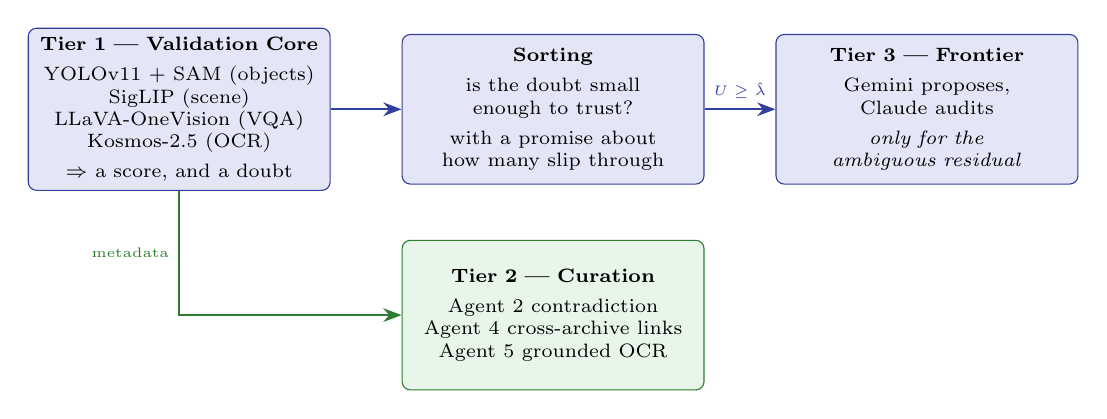
\begin{tikzpicture}[
  node distance=0.5cm and 0.9cm,
  box/.style={draw=HildesheimRed, fill=PrismLightBlue, rounded corners=3pt, align=center, text width=3.6cm, minimum height=1.9cm, font=\scriptsize},
  arrow/.style={->, >=Stealth, thick, HildesheimRed}]
\node[box] (t1) {\textbf{Tier 1 --- Validation Core}\\[1mm] YOLOv11 + SAM (objects)\\ SigLIP (scene)\\ LLaVA-OneVision (VQA)\\ Kosmos-2.5 (OCR)\\[1mm] $\Rightarrow$ a score, and a doubt};
\node[box, right=of t1] (tri) {\textbf{Sorting}\\[1mm] is the doubt small\\ enough to trust?\\[1mm] with a promise about\\ how many slip through};
\node[box, right=of tri] (t3) {\textbf{Tier 3 --- Frontier}\\[1mm] Gemini proposes,\\ Claude audits\\[1mm] \emph{only for the}\\ \emph{ambiguous residual}};
\node[box, below=0.7cm of tri, fill=PrismLightGreen, draw=PrismGreen] (t2) {\textbf{Tier 2 --- Curation}\\[1mm] Agent 2 contradiction\\ Agent 4 cross-archive links\\ Agent 5 grounded OCR};
\draw[arrow] (t1) -- (tri);
\draw[arrow] (tri) -- node[above, font=\tiny]{$U\ge\hat\lambda$} (t3);
\draw[arrow, PrismGreen] (t1.south) |- node[pos=0.25, left, font=\tiny]{metadata} (t2.west);
\end{tikzpicture}
\vspace{2mm}

\footnotesize \textbf{Decoupling rule:} Tier~2 enriches metadata \emph{after} routing and never feeds back into trust. Below $\hat\lambda$, images are catalogued automatically; above, they go onward.
\end{frame}

\begin{frame}{The Data, and the Number That Governs Everything}
\small
\begin{center}
\footnotesize
\begin{tabular}{@{}l r l@{}}
\toprule
\textbf{Set of images} & \textbf{How many} & \textbf{What it is for} \\
\midrule
The whole archive subset & $12{,}110$ & every model runs on all of these \\
Checked by an expert & $801$ & building and tuning the system \\
Checked and corrected & $1{,}250$ & judging the system fairly \\
\quad of those, kept aside for the final test & $249$ & never used while building \\
Pages confirmed to show no scene & $319$ & finding the blind spot \\
Waiting to be labelled & $465$ & prepared, not yet done \\
\bottomrule
\end{tabular}
\end{center}
\vspace{3mm}

\begin{alertblock}{\small The one number to remember}
\footnotesize Only about \textbf{one picture in eight} has ever been looked at by a person. Every claim about accuracy in this thesis is measured on that eighth --- and mostly on the small set kept aside for the final test. \textbf{That, not computing power, is what limits this work.}
\end{alertblock}
\end{frame}


\section{Where It Works}

\begin{frame}{Where It Works --- in One Sentence}
\large
The part of this thesis that survives is the \textbf{routing}: deciding which pictures a human must see.
\vspace{4mm}

It comes with a mathematical guarantee --- \emph{``of everything I approve without you, no more than $5\%$ will be wrong''} --- and that guarantee held on every partition I tested.
\vspace{4mm}

\normalsize It also runs at full archive scale, and every number in this deck can be regenerated from a single command.
\end{frame}


\begin{frame}{It Spots Its Own Mistakes --- on Pages That Have a Scene}
\normalsize
On a picture that really does show a scene, the system is good at knowing when it has got the answer wrong.
\vspace{3mm}

\small
If you lined up all the pictures it got wrong and all the pictures it got right, and asked it to sort them, it would put almost all the wrong ones first.
\vspace{4mm}

\normalsize
\textbf{On a picture with no scene, it cannot do this at all.}
\vspace{2mm}

\small
Pages with no scene --- printed text, sheet music, decoration --- are the ones it gets wrong most confidently. All four models agree with each other, and all four are wrong together. There is no disagreement to notice.
\vspace{4mm}

\begin{alertblock}{\small This is the honest boundary of the method}
It works where there is something to see. It fails where there is nothing to see --- and those are exactly the pictures a curator would most like flagged.
\end{alertblock}
\end{frame}

\begin{frame}{The Promise It Can Make, and Keep}
\normalsize
This is the part I would defend hardest.
\vspace{3mm}

\small
The system sorts pictures into two piles: \textbf{``catalogue automatically''} and \textbf{``a person should look''}, and makes a promise about the first pile:
\vspace{2mm}

\begin{exampleblock}{\normalsize The promise}
\normalsize ``Of every hundred pictures I catalogue without you, no more than five will be wrong.''
\end{exampleblock}
\vspace{3mm}

\small
That is not a hope or an average from past runs. It comes from a method that assumes nothing about the models or the images. \textbf{I tested it on pictures the system had never seen, and it held.}
\vspace{2mm}

At that promise, about \textbf{six pictures in ten} are catalogued automatically, and \textbf{nine mistakes in ten} still reach a person.
\end{frame}

\begin{frame}{Anyone Can Check My Work}
\normalsize
Every number in this thesis can be regenerated from the raw model outputs.
\vspace{4mm}

\small
\begin{itemize}
  \setlength\itemsep{2mm}
  \item \textbf{Thirty-six experiments} each carry a self-check. Run them all and every one reproduces its published figures.
  \item There is a single worksheet that walks from the raw scans to every table in the thesis. It takes about ten minutes on a normal machine, with no paid services.
  \item The full model run --- all four models over all the images --- is scripted and can be repeated overnight.
\end{itemize}
\vspace{4mm}

\begin{block}{\small Why I spent time on this}
Twice this year I found that a number I had reported was wrong. Both times it was this checking that caught it, not a reviewer. It is the reason I trust the rest.
\end{block}
\end{frame}

\begin{frame}{The Whole Archive, Run for Real}
\normalsize
Until this month, some of my signals were read from a stored table rather than produced by the models.
\vspace{4mm}

\small
This month I ran all four models over every one of the twelve thousand pictures --- about four and a half hours on our four GPUs. It is the first time the system has genuinely been what I describe in the thesis.
\vspace{4mm}

Then I rebuilt the whole pipeline on those real outputs and re-measured everything.
\vspace{4mm}

\begin{block}{\small What that run bought}
\small It did not change the direction of any conclusion. What it changed is that I can now say ``the four models were actually run'' without a footnote --- and it is what turned up most of the problems in the next section.
\end{block}
\end{frame}





\section{Where It Fails}

\begin{frame}{Where It Fails --- in One Sentence}
\large
The idea the thesis is named for --- that \textbf{models disagreeing} tells you where the mistakes are --- does not hold.
\vspace{4mm}

\normalsize I did not accept that quickly. I found eight separate defects that could each have been the cause, fixed every one, and re-measured. The gap never closed; usually it got wider.
\vspace{4mm}

I also found several results thinner than they first looked, and one signal that had been running \emph{backwards} for the entire project.
\vspace{4mm}

\textbf{The slides that follow are me showing each of those, with the evidence.}
\end{frame}


\begin{frame}{Why the Idea Should Have Worked}
\small
The idea is not exotic. It is how ensembles are normally used.
\vspace{1.5mm}

\small
If four independent models look at the same picture and all say the same thing, that is a picture we can trust. If they pull in different directions, something about the picture is hard --- and a person should look at it.
\vspace{2mm}

This has a respectable pedigree: query-by-committee, deep ensembles, Bayesian active learning. It works in many domains.
\vspace{2mm}

\begin{block}{\small What it requires to work}
It needs two things to be true, and I checked neither at the start:
\vspace{2mm}
\begin{enumerate}
  \item the four models must be genuinely \textbf{measuring different things};
  \item they must sometimes \textbf{reach different conclusions}, not just differ in enthusiasm.
\end{enumerate}
\end{block}
\end{frame}

\begin{frame}{What Was Actually Happening}
\small
Neither condition held --- and it took me most of this month to see why.
\vspace{2mm}

\small
\textbf{The four signals were not four opinions.} One of them was built by subtracting two of the others, so it carried no new information at all. A second was so nearly constant that it was really measuring the shape of the questions I had asked, not the picture. A third counted how \emph{much} text the OCR model produced, not whether any of it was real.
\vspace{2mm}

\textbf{And the committee never actually disagreed.} Once each model's output is put on a common probability scale, every one of them says ``yes, there is a scene'' on essentially every picture. The archive is overwhelmingly scene-positive, so a model with weak evidence still leans positive.
\vspace{2mm}

So the ``disagreement'' I was measuring was not disagreement about the \emph{answer}. It was disagreement about how \emph{emphatically} they all agreed.
\end{frame}

\begin{frame}{The One That Was Running Backwards}
\small
The most useful thing I found this month was an outright mistake.
\vspace{2mm}

\small
The scene classifier is asked five questions --- is this a teaching scene, a family scene, a playing scene, a landscape, a drawing? --- and I took whichever scored highest as ``how scene-like is this picture''.
\vspace{1.5mm}

\textbf{But all five questions name a kind of scene.} Forcing a choice among them can never produce the answer ``none of these --- this picture has no scene in it''. The model was made to pick a favourite even when it believed none applied.
\vspace{2mm}

The model's own honest answer was sitting in the output the whole time, computed for every picture and never read. Read correctly, the same model goes from \emph{worse than guessing} to genuinely useful.
\vspace{2mm}

\begin{alertblock}{\small Why this matters beyond the bug}
It is a reminder that a signal can look healthy --- it varied, it correlated sensibly, it passed every check I ran --- and still be pointed the wrong way.
\end{alertblock}
\end{frame}

\begin{frame}{Why Fixing Everything Did Not Rescue the Idea}
\small
I found eight separate defects. Each was real. I fixed every one and measured again.
\vspace{2mm}

\small
The derived signal, the constant signal, the miscounted signal, the backwards signal, the coarse discretisation, the circular way I was defining ``error'', and finally the unanimity itself --- I forced the models apart so they genuinely could disagree.
\vspace{2mm}

\textbf{The gap never closed. In most cases it got wider.}
\vspace{2mm}

And the last fix is the one that settles it. In the single configuration where all four models genuinely reach different conclusions about the same picture, their disagreement predicts mistakes \textbf{no better than a coin flip}.
\vspace{2mm}

\begin{alertblock}{\small The sentence I would put in the abstract}
Disagreement is not uninformative because the models never disagree. It is uninformative \emph{when they do}.
\end{alertblock}
\end{frame}

\begin{frame}{Why That Is a Structural Result, Not Bad Luck}
\small
Two ways of seeing why no amount of cleverness rescues this.
\vspace{2mm}

\small
\textbf{First, the arithmetic.} Whether a picture is judged correctly is decided by the \emph{average} of the signals crossing a line. Disagreement is a measure of \emph{spread}, which is deliberately built to ignore the average. I was asking a question designed not to hear the answer.
\vspace{2mm}

\textbf{Second, exhaustion.} For the deployed system I enumerated every possible way of ranking the states the signals can reach --- all forty thousand of them --- and the best conceivable one barely beats simply asking the system how confident it was. For the rebuilt system, where enumeration is impossible, I let models fit directly on the test data, which is cheating, and they still lost.
\vspace{2mm}

\textbf{There is no formula left to try.} That is worth more than another inconclusive comparison.
\end{frame}

\begin{frame}{The Thing That Did Work}
\small
The fix came from taking the failures seriously rather than adding another model.
\vspace{2mm}

\small
Our own annotation work had already told us what the system's mistakes look like: it calls pictures of printed text, sheet music and decorative borders ``scenes''. Those are the errors.
\vspace{1.5mm}

And nothing in the system could \emph{express} that. Every signal measured how much a picture looked like a scene; none measured how much it looked like a non-scene.
\vspace{2mm}

\textbf{So I told it what a non-scene is} --- a page of printed text, sheet music, an ornamental border, a blank page, a title page, a table, a map --- and scored each picture against both lists.
\vspace{2mm}

\begin{exampleblock}{\small The only change in this thesis whose improvement is bigger than the noise}
No new model, no new inference, no new labelling. The image representations were already computed; seven short phrases had to be typed. It now flags roughly four out of five text-only pictures.
\end{exampleblock}
\end{frame}

\begin{frame}{And Several Results Are Thinner Than They Looked}
\small
Three I would rather tell you than have an examiner find.
\vspace{2mm}

\small
\textbf{The headline guarantee rests on very few mistakes.} The risk bound holds, but the test set contains only a handful of errors in the band that matters. It is true and it is fragile, and more labelled pictures is the only thing that fixes it.
\vspace{1.5mm}

\textbf{The calibration does not travel.} Probabilities that are almost perfectly calibrated within one group of volumes drift substantially when applied to volumes they were not calibrated on. The guarantee is only as good as the match between calibration and deployment.
\vspace{1.5mm}

\textbf{Two decision rules exist in the codebase}, differing on a knife-edge case that affects a couple of thousand pictures. One is right; the other is a rounding artefact. I found this, and it needs a decision.
\vspace{2mm}

\textbf{And the title promises more than I can evidence} --- which is its own slide in a moment.
\end{frame}



\section{What We Should Do}

\begin{frame}{What We Should Do --- the Shape of It}
\small
Four decisions. Two are mine to propose and yours to approve; two are genuinely yours.
\vspace{2mm}

\small
\begin{enumerate}
  \setlength\itemsep{1.5mm}
  \item \textbf{The system} --- what to change, remove and keep. I have measured all of it.
  \item \textbf{The thesis} --- how to frame a central mechanism that failed.
  \item \textbf{The title} --- it promises more than the evidence carries.
  \item \textbf{The time} --- four weeks, and exactly what they buy.
\end{enumerate}
\end{frame}

\begin{frame}{1. What to Change in the System}
\tiny
\begin{center}
\begin{tabular}{@{}l l p{7.0cm}@{}}
\toprule
\textbf{Component} & \textbf{Do this} & \textbf{Why} \\
\midrule
scene classifier & \textbf{Fix} & Read the model's honest answer instead of forcing a choice among five scene types. One line; turns a below-chance signal into a useful one. \\
\addlinespace
fusion weights & \textbf{Refit} & They were hand-set around a signal that was running backwards. The data wants the scene term to carry the most weight, not the least. \\
\addlinespace
agreement term & \textbf{Remove} & Arithmetic on two other signals. Repairing it so it genuinely compares two models makes it \emph{less} useful --- what made it look useful was the leak. \\
\addlinespace
VLM term & \textbf{Keep, demote} & Near useless for spotting errors, but it helps the scene decision. Keep it in the blend; stop calling it an opinion. \\
\addlinespace
OCR term & \textbf{Repair, relocate} & The repaired version measures whether the text is real. That belongs to the transcription agent, not the trust score. \\
\addlinespace
negative evidence & \textbf{Add} & The missing piece. Tell the system what a non-scene looks like. \\
\addlinespace
disagreement & \textbf{Retire} & Fourteen formulations, two ceilings. Route on confidence --- it clears six times more of the archive at the same risk. \\
\bottomrule
\end{tabular}
\end{center}
\vspace{1mm}
\begin{exampleblock}{\scriptsize All seven are implemented and measured}
\scriptsize Not proposals --- each change is made, run over the whole corpus, and verified. The evidence for every row is in the appendix.
\end{exampleblock}
\end{frame}

\begin{frame}{2. How I Think the Thesis Should Be Framed}
\small
Not as a system paper with a disappointing result. As a \textbf{methodological one}.
\vspace{2mm}

\small
The claim that cross-modal disagreement detects errors is plausible, is in the literature, and is what I set out to demonstrate. Establishing carefully that it \emph{does not hold} on a real archive --- and showing exactly why --- is a finding other people can use.
\vspace{2mm}

What makes it defensible rather than an excuse is the shape of the evidence:
\vspace{2mm}
\begin{itemize}
  \setlength\itemsep{1mm}
  \item eight independent defects, each a plausible cause, each fixed and re-measured;
  \item two exhaustive ceilings showing no formulation can win;
  \item a validation requirement for the pseudo-labelling literature that this archive makes visible.
\end{itemize}
\vspace{1.5mm}

\textbf{And the engineering still stands:} a routing mechanism with a guarantee that holds, at archive scale, fully reproducible.
\end{frame}

\begin{frame}{3. The Title --- I Think It Overclaims}
\small
\emph{``Multi agent systems for image analysis: object and complex scene detection''}
\vspace{2mm}

\small
Two problems, and I would rather raise them than have an examiner do it.
\vspace{1.5mm}

\textbf{``Object detection''} --- what the system actually uses is a count of objects, capped at three, taken from a language model's answer. Where I do evaluate real detection against human-drawn boxes, it is weak.
\vspace{1.5mm}

\textbf{``Complex scene detection''} --- every result in the thesis is evaluated as a binary question: is there a scene here or not. The five scene categories exist, but one of them accounts for three-quarters of the labelled examples and another has seven. No multi-class result can honestly be reported.
\vspace{2mm}

\begin{block}{\small What I suggest}
Keep the subtitle, which describes the real contribution accurately, and either retitle the main line to match the evidence, or add an explicit scope statement saying what ``detection'' means here. \textbf{I would like your view on which.}
\end{block}
\end{frame}

\section{Summary and Proposal}

\begin{frame}{Where That Leaves Me}
\large
I have a system that routes reliably, a guarantee that holds, and a corpus-scale reproducible pipeline.
\vspace{3mm}

I also have a central claim that failed, established more carefully than most positive results are.
\vspace{4mm}

\normalsize My view is that the second of those is worth more than it looks, and that the honest version of this thesis is stronger than the one I set out to write.
\vspace{3mm}

\textbf{But that is a judgement for you, not me --- which is why I wanted this meeting before I finish.}
\end{frame}


\begin{frame}{Scorecard --- What Holds and What Does Not}
\small
\begin{columns}[T]
\column{0.48\textwidth}
\begin{exampleblock}{\small What holds}
\footnotesize
\begin{itemize}
  \setlength\itemsep{1.2mm}
  \item It spots its own mistakes on pictures that show a scene
  \item The promise about the automatic pile is kept
  \item Every result can be re-run and comes out the same
  \item The rebuilt system, on real model outputs, still works
  \item The pictures I labelled look like the archive as a whole
\end{itemize}
\end{exampleblock}

\column{0.48\textwidth}
\begin{alertblock}{\small What does not}
\footnotesize
\begin{itemize}
  \setlength\itemsep{1.2mm}
  \item Disagreement does not beat simple confidence --- and cannot, in any form
  \item It is blind on pictures with no scene, which are the ones that matter most
  \item Three of the four signals were not measuring what their names said
  \item Calibration does not survive a move to new volumes
  \item Two decision rules exist and disagree
  \item Tier 2 gives the triage no support
\end{itemize}
\end{alertblock}
\end{columns}
\end{frame}

\begin{frame}{What the Thesis Actually Gives You}
\small
\begin{columns}[T]
\column{0.48\textwidth}
\begin{exampleblock}{\small A system that works, with a promise attached}
\footnotesize Most of an archive catalogued automatically, with a stated limit on how many errors slip through unchecked --- tested on volumes it had never seen, and reproducible by anyone.
\end{exampleblock}
\vspace{1mm}
\begin{exampleblock}{\small A settled question, not a failed try}
\footnotesize Not ``I tried nine things and none worked''. I can show that \emph{nothing} built from these signals can do better than simply asking the system how sure it is.
\end{exampleblock}

\column{0.48\textwidth}
\begin{block}{\small A clear account of why the idea failed}
\footnotesize The system works, but not for the reason I proposed. Three of the four signals were not independent opinions, and the models almost never actually disagreed.
\end{block}
\vspace{1mm}
\begin{block}{\small A warning other people can use}
\footnotesize A model graded by its own teacher looked nearly perfect and was not. A pool of unchecked labels reversed a finding. \textbf{Checking the evaluation mattered more than improving the model.}
\end{block}
\end{columns}
\end{frame}

\begin{frame}{What Four More Weeks Would Buy}
\small
Some of my experiments still run on the old stored signals rather than the real model outputs. I would like to finish that properly.
\vspace{2mm}
\begin{center}
\scriptsize
\renewcommand{\arraystretch}{1.0}
\begin{tabular}{@{}c p{5.6cm} p{5.6cm}@{}}
\toprule
\textbf{Week} & \textbf{What I would do} & \textbf{What you would get} \\
\midrule
1 & Finish labelling the pictures waiting for review & A real estimate of the deployment risk, instead of one resting on a handful of cases \\
2 & Settle the two decision rules into one & A single set of results, with no footnote \\
3 & Re-run the remaining experiments on the real model outputs & A results chapter built entirely on measured inputs \\
4 & Re-check everything, revise, rebuild the defence materials & A final thesis and deck \\
\bottomrule
\end{tabular}
\end{center}
\vspace{1mm}
\begin{alertblock}{\small Why not simply list these as limitations}
\footnotesize I could defend now and note them --- but I would be defending a promise thinner than it sounds, on inputs I have shown were not what I described. \textbf{These weeks change what I can claim.}
\end{alertblock}
\end{frame}




\begin{frame}{Questions I Expect, and My Answers}
\tiny
\begin{center}
\begin{tabular}{@{}p{5.0cm} p{7.4cm}@{}}
\toprule
\textbf{What you may well ask} & \textbf{My answer} \\
\midrule
\emph{``You already told us disagreement fails. What is new?''} & The draft asserted it from one comparison. I now have nine formulations, an exhaustive proof over every reachable ranking, and eight separate defects each fixed and re-measured. It went from a result to a bound. \\
\addlinespace
\emph{``Your scene signal was wrong the whole time. How much else is wrong?''} & Fair, and I do not know what I have not found. What I can show is the method that found it --- every experiment carries a reproducibility check and a full sweep passes. That bug was caught by that discipline. \\
\addlinespace
\emph{``Does correcting it change any conclusion?''} & No. It makes the pipeline better and the negative result \emph{stronger} --- the gap widened. If it had rescued disagreement I would be telling you the opposite. \\
\addlinespace
\emph{(Prof.\ Mandl)} \emph{``You position against my 2024 paper. On what grounds?''} & Not on results --- on protocol. Pseudo-labelling is scored against a held-out split of the same pseudo-labelled distribution. Run both on one model: nearly perfect against the teacher, roughly one in seven against a person. A validation requirement, not a refutation. \\
\addlinespace
\emph{``So is your detection any good?''} & No, and I do not claim it is. That is why I am raising the title. \\
\addlinespace
\emph{``Is a negative result a thesis?''} & Genuinely your call. My case: the engineering deliverable stands and is certified, and the negative result is established more carefully than most positive ones. \\
\bottomrule
\end{tabular}
\end{center}
\end{frame}

\begin{frame}{The One Thing I Would Ask You to Weigh}
\small
Every number in this thesis now rests on \textbf{249 test images}, of which \textbf{38} contain no scene.
\vspace{3mm}

That is the real limit. Not compute --- I have four GPUs and the whole corpus runs overnight. Not method --- the pipeline is reproducible end to end.
\vspace{4mm}

\small
It is why the improvement I found cannot be proven as firmly as I would like, and why the blind-spot result moved twice as the labels were corrected.
\vspace{3mm}

\textbf{Of everything four more weeks could buy, labelled pictures are worth the most} --- and $465$ are already prepared and waiting.
\vspace{3mm}

\small If you tell me to defend now instead, that is the sentence I would put in the limitations: \emph{the evidence is thin in exactly one dimension, and it is the one I could not buy with compute.}
\end{frame}

\begin{frame}{Questions for You}
\begin{enumerate}
  \setlength\itemsep{4mm}
  \item \textbf{Is four weeks acceptable?} Or would you prefer I defend now with these documented as limitations?
  \item \textbf{The negative result is the core finding.} Is a thesis whose central mechanism fails --- but is shown to fail rigorously --- the thesis you want me to defend?
  \item \textbf{The two decision rules.} Reconcile them (re-deriving every downstream number), or document and leave?
  \item \textbf{Tier 3.} Is there any budget for frontier API calls, or should it stay formally untested?
  \item \textbf{Scope.} Anything here you would cut rather than extend?
\end{enumerate}
\end{frame}

\appendix
\section{Appendix --- Reference Material}

\begin{frame}[standout]
Reference material
\vspace{4mm}

{\normalsize Everything from here on is backup: the formulas, the algorithms, and the full experiment record.\\[2mm]
It is here to answer questions, not to be presented.}
\end{frame}

\section{Evidence for Each Finding}

\begin{frame}{How to Read Every Number in This Deck}
\small
Four quantities carry almost every claim that follows. Each is stated plainly here once, so the tables later need no explaining.
\vspace{1mm}
\begin{center}
\tiny
\begin{tabular}{@{}l p{8.7cm}@{}}
\toprule
\textbf{Quantity} & \textbf{What it actually asks} \\
\midrule
\textbf{ROC-AUC} & Take one image the system got \emph{wrong} and one it got \emph{right}. How often does the score rank the wrong one as more suspicious? \\
& \quad $1.00$ = always \quad $0.50$ = \textbf{a coin flip} \quad $<0.50$ = \textbf{pointing the wrong way} \\
\addlinespace
\textbf{Balanced accuracy} & The average of ``how many scenes did we find'' and ``how many pictures with no scene did we correctly leave alone''. $0.50$ is a coin flip. Used instead of plain accuracy because $84.5\%$ of images contain a scene --- always guessing ``scene'' scores $84.5\%$ and is worthless. \\
\addlinespace
\textbf{$95\%$ confidence interval} & The range the number would land in if the experiment were repeated. If it \textbf{excludes zero}, the difference is real rather than noise. If it \textbf{spans zero}, we cannot tell the two apart. \\
\addlinespace
\textbf{Error rate} & The fraction of the $249$ test images where the system's scene / no-scene call disagreed with the human label. \\
\bottomrule
\end{tabular}
\end{center}
\vspace{1mm}
\begin{alertblock}{\small One number governs all of them}
\footnotesize $\mathbf{n=249}$. That is the whole held-out test set, and it contains only $\mathbf{38}$ images with no scene. Every certified figure in this deck rests on those $249$ images, and every interval is as wide as it is because of them.
\end{alertblock}
\end{frame}
\begin{frame}{Fails: Disagreement Does Not Beat Plain Confidence}
\begin{columns}[T]
\column{0.5\textwidth}
\small
The thesis's core idea was that \emph{disagreement} between models signals doubt. Tested directly, it does not outperform the simplest baseline --- the pipeline's own confidence, $1 - SAA$.
\vspace{1mm}
\begin{center}
\footnotesize
\begin{tabular}{@{}l r@{}}
\toprule
\textbf{Held-out, $n=249$} & \textbf{ROC-AUC} \\
\midrule
\textbf{Ceiling} (any function) & $\mathbf{0.8871}$ \\
plain confidence & $0.8828$ \\
learned, $A^{\text{agree}}$ dropped & $0.8801$ \\
deployed $U_{\text{SAA}}$ & $0.8600$ \\
\bottomrule
\end{tabular}
\end{center}

\column{0.46\textwidth}
\begin{alertblock}{\small Why no formulation can win}
\footnotesize Only 8 signal states exist, so \emph{any} function of them is constant within a state. Its ranking is fixed by how it orders 8 states. I evaluated all $8! = 40{,}320$ orderings: the best reaches $0.8871$.
\vspace{1mm}

Confidence sits \textbf{$0.0043$} below that ceiling. No weighting, nonlinearity or classifier over these signals can beat it by more.
\end{alertblock}
\vspace{1mm}
\footnotesize Nine formulations were also tried directly. All fell below confidence.
\end{columns}
\end{frame}
\begin{frame}{Fails: And Redesigning the Signals Makes It Worse}
\scriptsize
The obvious repair: stop crushing the outputs. Use the detector's confidence, and the classifier's full distribution over the five scene categories.
\vspace{1mm}
\begin{center}\scriptsize
\begin{tabular}{@{}l r r@{}}
\toprule
& \textbf{Deployed} & \textbf{Redesigned} \\
\midrule
$A^{\text{object}}$: $\min(k/3,1)$ $\rightarrow$ detector max confidence & $4$ values & $\mathbf{8{,}979}$ \\
$A^{\text{scene}}$: binary flag $\rightarrow$ softmax over 5 categories & $2$ values & $\mathbf{11{,}882}$ \\
$A^{\text{vlm}}$: one bit $\rightarrow$ fraction of 10 classes named & $2$ values & $7$ \\
$U_{\text{SAA}}$ & $8$ values & $\mathbf{1{,}247}$ \\
\bottomrule
\end{tabular}
\end{center}
\vspace{-1mm}
\begin{center}\scriptsize
\begin{tabular}{@{}l c c c@{}}
\toprule
\textbf{Signal set} & \textbf{disagreement} & \textbf{confidence} & \textbf{gap (95\% CI)} \\
\midrule
Deployed & $0.8600$ & $0.8828$ & $-0.023$ \\
Redesigned, max softmax & $0.5547$ & $\mathbf{0.8324}$ & $\mathbf{-0.278}$ $[-0.36,-0.20]$ \\
Redesigned, peakedness & $0.6273$ & $\mathbf{0.8430}$ & $\mathbf{-0.216}$ $[-0.29,-0.14]$ \\
\bottomrule
\end{tabular}
\end{center}
\vspace{-2mm}
\begin{alertblock}{\scriptsize The reduction was never the problem}
\scriptsize Given full resolution the gap \emph{widens} from $0.023$ to $0.22$--$0.28$, both intervals below zero. A richer $SAA$ is a better estimate of whether the pipeline is right; its spread is not. \textbf{Not a deployment proposal} --- the redesign is worse in balanced accuracy ($0.66$--$0.68$ vs $0.78$).
\end{alertblock}
\end{frame}
\begin{frame}{Fails: A Shared Blind Spot on True Negatives}
\small
On images a human confirms contain \emph{no} scene, all models agree the image shows something --- and all are wrong. Disagreement stays low exactly where a warning is most needed.
\vspace{1mm}
\begin{center}
\footnotesize
\begin{tabular}{@{}l c c c c@{}}
\toprule
\textbf{Pool} & $\bm n$ & \textbf{errors} & \textbf{ROC-AUC} & \textbf{95\% CI} \\
\midrule
Original held-out & $38$ & $5$ & $0.1152$ & $[0.000,\,0.396]$ \\
New, disjoint annotation pass & $123$ & $27$ & $0.1852$ & $[0.080,\,0.306]$ \\
\textbf{All confirmed negatives} & $\mathbf{319}$ & $\mathbf{50}$ & $\mathbf{0.1259}$ & $[0.062,\,0.196]$ \\
\bottomrule
\end{tabular}
\end{center}
\vspace{1mm}
\begin{alertblock}{\small Replicated --- and partly explained}
\footnotesize The finding survived an independent annotation pass. But a quarter of the gap to chance is \emph{arithmetic}: on a true negative an error needs $SAA\ge0.5$, impossible when $A^{\text{object}}=0$ --- and that is exactly where $A^{\text{agree}}$ jumps to 1. The rest is a genuine failure.
\end{alertblock}
\end{frame}
\begin{frame}{Fails: Two Signals Were Not What They Claimed}
\begin{columns}[T]
\column{0.48\textwidth}
\begin{alertblock}{\small 1. The object signal was a fallback}
\footnotesize The fusion code:
\vspace{1mm}

{\tiny\texttt{if student\_count <= 0:}\\\texttt{\ \ student\_count = vqa\_total\_objects}}
\vspace{1mm}

\texttt{student\_v3\_count} is \textbf{zero on all $12{,}110$ rows}, so the branch always fires. The detector only ever ran on \textbf{$231$} images.
\vspace{1mm}

Confirmed by running both code paths: only the fallback path regenerates the thesis's table.
\end{alertblock}

\column{0.48\textwidth}
\begin{alertblock}{\small 2. The VLM signal is near-constant}
\footnotesize $A^{\text{vlm}}$ = fraction of 4 VQA questions answered in $\ge 3$ words.
\vspace{1mm}

But two questions are yes/no by design:
\vspace{1mm}
\begin{center}
\begin{tabular}{@{}l r@{}}
q0, q1 (descriptive) & $100\%$, $99.9\%$ \\
q2, q3 (yes/no) & $0\%$, $1\%$ \\
\end{tabular}
\end{center}
\vspace{1mm}
So it equals $2/4$ on \textbf{$98.9\%$} of images. It encodes the question format, not the image. \emph{Found only by running the model.}
\end{alertblock}
\end{columns}
\end{frame}
\begin{frame}{Fails --- and the Fix Does Not Rescue It}
\small
The obvious objection: \emph{``your negative result is an artifact of the fallback.''} This week made that testable.
\vspace{1mm}
\begin{center}
\footnotesize
\begin{tabular}{@{}l r r@{}}
\toprule
& \textbf{Deployed (fallback)} & \textbf{Rebuilt (real inference)} \\
\midrule
$U_{\text{SAA}}$ distinct values & $8$ & $\mathbf{11{,}786}$ \\
$A^{\text{vlm}} = \mathbb{I}[A^{\text{object}}>0]$ & $100\%$ & $78.9\%$ \\
disagreement ROC-AUC & $0.8600$ & $0.8098$ \\
confidence ROC-AUC & $0.8828$ & $0.8483$ \\
\bottomrule
\end{tabular}
\end{center}
\vspace{1mm}
\begin{alertblock}{\small Result}
\footnotesize With every signal measured by a real model, the derived term a genuine comparison, and the 8-state discretisation gone --- \textbf{disagreement still trails confidence} ($-0.039$, CI $[-0.083,\,0.005]$). The negative result is not an artifact of the defect.
\end{alertblock}
\end{frame}
\begin{frame}{Fails: Three Signals Do Not Measure What They Are Named For}
\small
A separate question from ``is the formulation right'': do the signals measure the quantity their \emph{names} claim? Three of four do not.
\vspace{1mm}
\begin{center}
\scriptsize
\begin{tabular}{@{}l p{3.5cm} p{4.3cm}@{}}
\toprule
& \textbf{What it is} & \textbf{Repaired to measure its name} \\
\midrule
$A^{\text{agree}}$ & arithmetic on two numbers; $=1-|A^{\text{obj}}-\tfrac12|$ on $\mathbf{98.9\%}$ & Jaccard overlap of the detector's label \emph{set} and the VLM's named-class \emph{set} \\
\addlinespace
$A^{\text{ocr}}$ & $\min(\text{chars}/80,1)$: text \emph{volume} & $(1-\text{repetition})\times\text{wordlikeness}$ \\
\addlinespace
$A^{\text{vlm}}$ & fraction of answers $\ge 3$ words & fraction of the 10 taxonomy classes named \\
\bottomrule
\end{tabular}
\end{center}
\vspace{1mm}
\begin{alertblock}{\small Why this survived every check}
\footnotesize $A^{\text{agree}}$ correlates with $A^{\text{object}}$ at only $r=0.18$. The dependence is \textbf{exact but not linear}, so a correlation screen passes it. It also has $8{,}984$ distinct values --- more than any other signal --- and is still a deterministic function of one of them. Resolution is not information.
\end{alertblock}
\end{frame}
\begin{frame}{The OCR Repair Works --- and Changes Nothing for Trust}
\small
Rebuilt for all $12{,}110$ images from outputs that already existed.
\begin{columns}[T]
\column{0.46\textwidth}
\begin{exampleblock}{\small The repair that works}
\footnotesize Deployed $A^{\text{ocr}}$ saturates at $1.0$ on $\mathbf{68.6\%}$ of images. Repaired score on those same images: $\mathbf{0.159}$ vs $0.378$ elsewhere. Correlation between them: $\mathbf{-0.32}$.
\vspace{1mm}

{\tiny\texttt{\# ONE / \#\# ONE / \#\#\# ONE / \ldots}\\ deployed $1.000$ $\rightarrow$ repaired $0.007$}
\end{exampleblock}

\column{0.5\textwidth}
\begin{center}
\scriptsize ROC-AUC against the shipped rule's errors\\($n=249$, $90$ errors)
\vspace{1mm}

\begin{tabular}{@{}l c c@{}}
\toprule
& \textbf{deployed} & \textbf{repaired} \\
\midrule
$A^{\text{object}}$ & \multicolumn{2}{c}{$\mathbf{0.854}$} \\
$A^{\text{agree}}$ & $0.684$ & $0.577$ \\
$A^{\text{vlm}}$ & $0.501$ & $0.566$ \\
$A^{\text{ocr}}$ & $0.531$ & $0.478$ \\
\midrule
confidence & \multicolumn{2}{c}{$\mathbf{0.850}$} \\
\bottomrule
\end{tabular}
\end{center}
\end{columns}
\vspace{1mm}
\begin{alertblock}{\small The decisive number}
\footnotesize Confidence alone $0.8499$ $\rightarrow$ confidence $+$ all three repaired signals $0.8563$. Difference $\mathbf{+0.006}$, CI $[-0.004,+0.018]$ --- \textbf{spans zero}, under every decision rule tested.
\end{alertblock}
\end{frame}
\begin{frame}{Why Repairing Agreement Makes It Worse}
\small
Repairing the signal makes it \emph{less} predictive --- $0.684 \rightarrow 0.577$. That is not a failed repair; it is the diagnosis.
\vspace{2mm}
\begin{center}
\footnotesize
\begin{tabular}{@{}l c@{}}
\toprule
$U_{\text{SAA}}$ spread over \textbf{deployed} signals & $0.8558$ \\
$U_{\text{SAA}}$ spread over \textbf{repaired} signals & $\mathbf{0.4362}$ \\
confidence $1-SAA$ & $0.8499$ \\
\midrule
paired difference, repaired spread $-$ confidence & $-0.413$ \\
$95\%$ bootstrap CI & $[-0.513,\,-0.310]$ \\
\bottomrule
\end{tabular}
\end{center}
\vspace{2mm}
\begin{alertblock}{\small What this says}
\footnotesize The deployed spread worked because three of its four terms were \textbf{algebraic restatements of the fourth}, which made a standard deviation behave like a function of the level. Supply genuinely independent measurements and the coupling goes --- and so does the performance. The deployed $A^{\text{agree}}$ scored $0.684$ by being a copy of $A^{\text{object}}$, the one signal that does predict.
\end{alertblock}
\end{frame}
\begin{frame}{Plan: Remove Two, Relocate One}
\small
\begin{center}
\scriptsize
\begin{tabular}{@{}l l p{5.6cm}@{}}
\toprule
\textbf{Signal} & \textbf{Verdict} & \textbf{Why} \\
\midrule
$A^{\text{agree}}$ & \textbf{Remove} & Not repairable into a trust term. Also removes the asymmetry that reported near-maximal uncertainty where the ensemble was unanimously \emph{negative}. \\
\addlinespace
$A^{\text{ocr}}$ & \textbf{Relocate} & Keep the repair, move to Agent~5's bucket assignment, where validity is the question asked. Its chance-level $0.478$ against \emph{scene} errors is correct --- the two are unrelated quantities. \\
\addlinespace
$A^{\text{vlm}}$ & \textbf{Demote} & Carry the named-class \emph{set} to Tier~2 contradiction detection; drop the scalar from Tier~1. \\
\bottomrule
\end{tabular}
\end{center}
\vspace{1mm}
\begin{exampleblock}{\small What Tier 1 becomes}
\footnotesize Trust rests on $A^{\text{object}}$ and $A^{\text{scene}}$, ranked by \textbf{confidence, not spread}. Not a loss: at the same risk level, confidence triage certifies $\mathbf{61.1\%}$ of the corpus against $\mathbf{10.0\%}$ on spread, at higher error recall.
\end{exampleblock}
\end{frame}
\begin{frame}{The Root Cause: The Scene Agent Read the Wrong Channel}
\small
SigLIP is trained with a \textbf{sigmoid} objective --- each prompt gets an independent calibrated probability. The pipeline applied a \textbf{softmax} across five prompts that are \emph{all} scene types.
\vspace{1mm}
\begin{center}
\scriptsize
\begin{tabular}{@{}l c c@{}}
\toprule
& \textbf{softmax (deployed)} & \textbf{sigmoid (unused)} \\
\midrule
Minimum over the corpus & $0.2956$ & $\mathbf{0.0}$ \\
Can express ``no scene'' & \textbf{no} & \textbf{yes} ($48.6\%$ below $0.01$) \\
Correlation between them & \multicolumn{2}{c}{$-0.096$} \\
\midrule
\textbf{ROC-AUC vs.\ scene presence} & $\mathbf{0.4172}$ \emph{(below chance)} & $\mathbf{0.7754}$ \\
Learned fusion coefficient & $-0.162$ \emph{(subtract it)} & $+0.486$ \emph{(largest)} \\
\bottomrule
\end{tabular}
\end{center}
\vspace{1mm}
\begin{alertblock}{\small Both channels were computed in the same pass and stored for all 12,110 images}
\footnotesize A softmax over five scene types is a forced choice \emph{among} scenes. On the $5{,}887$ images SigLIP says match \emph{no} scene prompt, the deployed signal reports mean $0.84$ and exceeds $0.5$ on $95.2\%$. Paired gain $+0.358$, CI $[+0.299,+0.415]$.
\end{alertblock}
\end{frame}
\begin{frame}{Fixing It Helps the Pipeline --- and Kills the Last Hypothesis}
\small
\begin{columns}[T]
\column{0.44\textwidth}
\begin{exampleblock}{\small End to end ($n=249$)}
\scriptsize
\begin{tabular}{@{}l c c@{}}
\toprule
& \textbf{dep.} & \textbf{fixed} \\
\midrule
error rate & $42.6\%$ & $\mathbf{39.4\%}$ \\
bal.\ accuracy & $0.663$ & $\mathbf{0.682}$ \\
$SAA$ vs.\ scene & $0.722$ & $0.748$ \\
confidence & $0.832$ & $0.840$ \\
\bottomrule
\end{tabular}
\vspace{1mm}

{\tiny Signal-level gain is significant; the \emph{fused} gain is $+0.025$, CI $[-0.016,+0.066]$ --- $A^{\text{scene}}$ enters at weight $0.2$.}
\end{exampleblock}

\column{0.52\textwidth}
\begin{center}
\scriptsize Does breaking unanimity rescue disagreement?
\vspace{1mm}

\begin{tabular}{@{}l c c c@{}}
\toprule
& \textbf{unanim.} & \textbf{epist.} & \textbf{conf.} \\
\midrule
dep., unweighted & $100\%$ & $0.612$ & $0.804$ \\
dep., balanced & $11.2\%$ & $0.589$ & $0.799$ \\
fixed, unweighted & $100\%$ & $0.647$ & $0.831$ \\
\textbf{fixed, balanced} & $\mathbf{14.9\%}$ & $\mathbf{0.501}$ & $0.809$ \\
\bottomrule
\end{tabular}
\end{center}
\end{columns}
\vspace{1mm}
\begin{alertblock}{\small The decisive row}
\footnotesize The ensemble was unanimous on \textbf{100\%} of images --- an 84.5\% base rate, not a signal defect. Class-balanced calibration breaks it (unanimity $\rightarrow 14.9\%$). In the configuration where the models genuinely disagree, disagreement scores $\mathbf{0.5014}$ --- chance --- and the gap widens to $\mathbf{-0.307}$.
\end{alertblock}
\end{frame}
\begin{frame}{Eight Repairs, One Result}
\small
Every plausible cause of the negative result has now been identified, corrected, and re-measured.
\vspace{1mm}
\begin{center}
\scriptsize
\begin{tabular}{@{}l l@{}}
\toprule
\textbf{Defect corrected} & \textbf{Effect on the claim} \\
\midrule
1. Agreement term derived, not measured & gap persists \\
2. Object signal came from a fallback & gap persists ($0.810$ vs $0.848$) \\
3. VLM term near-constant ($2/4$ on $98.9\%$) & gap persists \\
4. OCR term measured volume, not validity & gap persists \\
5. Eight-valued discretisation & gap \textbf{widens} to $-0.278$ \\
6. Circular error label & gap persists (BALD, human labels) \\
7. \textbf{Scene channel read as softmax} & gap \textbf{widens} \\
8. \textbf{Ensemble unanimous on 100\%} & gap \textbf{widens} to $\mathbf{-0.307}$ \\
\bottomrule
\end{tabular}
\end{center}
\vspace{1mm}
\begin{exampleblock}{\small What this is worth}
\footnotesize A negative result that survives eight independent repairs --- each a real defect with a plausible claim to being the cause --- is far stronger than the single comparison the chapter opened with. \textbf{The repairs are the contribution}, not failed attempts to avoid the finding.
\end{exampleblock}
\end{frame}
\begin{frame}{The Fixes, Applied and Measured}
\small
All four corrections were carried out, not left as recommendations. The scene channel is now a parameter of every affected experiment --- the deployed figures stay reproducible, the corrected column sits beside them.
\vspace{1mm}
\begin{center}
\scriptsize
\begin{tabular}{@{}l c c c@{}}
\toprule
\textbf{Configuration} ($n=249$) & \textbf{Error rate} & \textbf{Bal.\ acc.} & \textbf{$SAA$ vs.\ scene} \\
\midrule
Deployed channel, hand-set $0.6/0.2/0.2$ & $42.2\%$ & $0.6649$ & $0.7222$ \\
Deployed channel, weights refitted & $37.8\%$ & $0.6909$ & $0.7387$ \\
Corrected channel, hand-set weights & $39.4\%$ & $0.6815$ & $0.7478$ \\
\textbf{Corrected channel, weights refitted} & $\mathbf{36.6\%}$ & $0.6873$ & $\mathbf{0.7599}$ \\
\bottomrule
\end{tabular}
\end{center}
\vspace{1mm}
\begin{block}{\small Refitting matters as much as the channel}
\footnotesize $0.6/0.2/0.2$ was hand-set around a signal running backwards. Refitted on the corrected channel it becomes $\mathbf{0.245/0.487/0.269}$ --- the scene agent goes from smallest weight to largest. Re-running the whole section on the corrected channel leaves every conclusion standing: the disagreement gap \emph{widens} from $-0.278$ to $\mathbf{-0.318}$.
\end{block}
\end{frame}
\begin{frame}{A Detector for the Error We Actually Make}
\small
The dominant failure is a false positive on a true negative --- printed text, sheet music, ornament. \textbf{None of the five prompts can name any of them.} So we said so: explicit \emph{negative} prompts, scored with SigLIP's own logit scale and bias.
\vspace{1mm}
\begin{columns}[T]
\column{0.5\textwidth}
\begin{center}
\scriptsize ROC-AUC vs.\ scene presence
\vspace{1mm}

\begin{tabular}{@{}l c@{}}
\toprule
deployed softmax & $0.4345$ \\
corrected sigmoid & $0.7188$ \\
\midrule
negative evidence alone & $0.8140$ \\
margin (scene $-$ neg.) & $0.8295$ \\
\textbf{fitted on both} & $\mathbf{0.8305}$ \\
\bottomrule
\end{tabular}
\end{center}

\column{0.46\textwidth}
\begin{exampleblock}{\small On true negatives}
\scriptsize mean negative evidence \\
\quad $0.390$ on true negatives \\
\quad $0.059$ on positives
\vspace{1mm}

flags $\mathbf{81.6\%}$ of true negatives, \\ $31.8\%$ of positives
\vspace{1mm}

test error rate $\mathbf{29.7\%}$ \\ {\tiny(vs $36.6\%$ corrected fusion, $42.2\%$ deployed)}
\end{exampleblock}
\end{columns}
\vspace{1mm}
\begin{alertblock}{\small The only result in this thesis whose interval excludes zero}
\footnotesize Against the \emph{corrected} baseline: $\mathbf{+0.111}$, CI $[+0.045,+0.181]$. Found by taking the failure analysis seriously, not by adding a model. Caveat: only $38$ true negatives in test.
\end{alertblock}
\end{frame}
\begin{frame}{Can the Formulation Itself Be Fixed? Yes --- Once}
\small
Repairing the signals changed nothing. Replacing one of them does. The deployed fusion had no term for the \emph{absence} of a scene.
\vspace{1mm}
\begin{equation*}
SAA^{\text{corrected}} = 0.192\,A^{\text{object}} + 0.500\,A^{\text{scene}} \;\mathbf{-}\; 0.308\,A^{\text{negative}}
\end{equation*}
\vspace{-2mm}
\begin{center}
\scriptsize
\begin{tabular}{@{}l c c c@{}}
\toprule
\textbf{Signal set} ($n=249$) & \textbf{error} & \textbf{bal.\ acc.} & \textbf{$SAA$ vs.\ scene} \\
\midrule
$A^{\text{object}}$ alone & $41.8\%$ & $0.6672$ & $0.7037$ \\
$A^{\text{object}} + A^{\text{scene}}$ ($A^{\text{vlm}}$ deleted) & $39.8\%$ & $0.6683$ & $0.7408$ \\
as deployed, corrected channel & $\mathbf{36.6\%}$ & $0.6873$ & $0.7599$ \\
\textbf{with the negative term} & $39.8\%$ & $\mathbf{0.7115}$ & $\mathbf{0.8231}$ \\
\bottomrule
\end{tabular}
\end{center}
\vspace{1mm}
\begin{exampleblock}{\small $+0.0631$, CI $[+0.0208,+0.1138]$ --- excludes zero}
\footnotesize And one correction to the premise: $A^{\text{vlm}}$ is near chance at ranking \emph{errors} ($0.569$), which is what made it look useless --- but \textbf{deleting it makes the fusion worse}. The two levels ask different questions of the same signal.
\end{exampleblock}
\end{frame}
\begin{frame}{And the Ceiling, Now for the Continuous Case}
\small
The $8!$ enumeration required $A^{\text{scene}}$ to have 2 values. Corrected, it has $1{,}520$ --- so the bound must be \emph{estimated} instead.
\vspace{1mm}
\begin{columns}[T]
\column{0.47\textwidth}
\begin{center}
\scriptsize Unsupervised operators vs.\ error
\vspace{1mm}

\begin{tabular}{@{}l c@{}}
\toprule
confidence $1-SAA$ & $\mathbf{0.8480}$ \\
\midrule
std over 5 signals & $0.2310$ \\
range (max $-$ min) & $0.2320$ \\
mean pairwise $|\Delta|$ & $0.2052$ \\
BALD epistemic & $0.4727$ \\
\bottomrule
\end{tabular}
\end{center}

\column{0.49\textwidth}
\begin{center}
\scriptsize Ceiling: fitted \emph{inside} the test split,\\held out only by publication
\vspace{1mm}

\begin{tabular}{@{}l c@{}}
\toprule
logistic & $0.8251$ \\
gradient boosting & $0.8391$ \\
random forest & $0.8362$ \\
\midrule
\textbf{confidence} & $\mathbf{0.8480}$ \\
\bottomrule
\end{tabular}
\end{center}
\end{columns}
\vspace{1mm}
\begin{alertblock}{\small An optimistic bound that still loses}
\footnotesize Those models see the test distribution during model selection, so they bound from \emph{above} what any learnable function of these signals can reach --- and none reaches confidence. That closes the continuous case as the enumeration closed the discrete one.
\end{alertblock}
\end{frame}
\begin{frame}{Fails: Calibration Does Not Transfer Across Publications}
\begin{columns}[T]
\column{0.5\textwidth}
\small
The thesis reports $\text{ECE} < 0.001$ after Platt scaling. That is fitted and scored on a \emph{random} $50\%$ split of $C_1$ --- where pictures from the same book fall on both sides.
\vspace{2mm}

On the PPN-disjoint split ($360$ training volumes, $79$ test, \textbf{none shared}):
\vspace{1mm}
\begin{center}
\footnotesize
\begin{tabular}{@{}l r@{}}
\toprule
& \textbf{ECE} \\
\midrule
reported (within-cohort) & $< 0.001$ \\
uncalibrated, disjoint & $0.116$ \\
Platt-scaled, disjoint & $\mathbf{0.109}$ \\
\bottomrule
\end{tabular}
\end{center}

\column{0.46\textwidth}
\begin{alertblock}{\small What it means}
\footnotesize The score \textbf{ranks} errors well across publications ($0.8828$) and is \textbf{not calibrated} across them.
\vspace{1mm}

A monotone recalibration cannot change ranking; what fails to transfer is the map from score to probability.
\vspace{1mm}

An institution relying on the stated \emph{probabilities} must recalibrate on its own holdings.
\end{alertblock}
\end{columns}
\end{frame}
\begin{frame}{Fails: Two Decision Rules, and a Knife-Edge}
\begin{columns}[T]
\column{0.48\textwidth}
\begin{alertblock}{\small A threshold on the seventh decimal}
\footnotesize One state, $(A^{\text{obj}},A^{\text{scn}},A^{\text{vlm}}) = (\tfrac13,\,0.5,\,1)$, lands exactly on the threshold:
\[
0.6\cdot\tfrac13 + 0.2\cdot0.5 + 0.2\cdot1 = 0.5
\]
$A^{\text{object}}$ is \emph{stored} as $0.333333$, so it computes to $\mathbf{0.4999998}$ --- negative by $2\times10^{-7}$.
\vspace{1mm}

This one cell holds \textbf{$2{,}217$ images} ($18.3\%$ of the corpus).
\end{alertblock}

\column{0.48\textwidth}
\begin{alertblock}{\small So two rules coexist}
\footnotesize A stored fusion column holds the exact $0.5$; recomputing from the agent columns gives $0.4999998$.
\vspace{1mm}

They disagree on \textbf{$2{,}217$ images}, and both produced numbers in the thesis:
\vspace{1mm}
\begin{center}
\begin{tabular}{@{}l r@{}}
same weights, same partition & \\
\quad recomputed rule & $70$ errors \\
\quad stored-column rule & $56$ errors \\
\end{tabular}
\end{center}
\end{alertblock}
\end{columns}
\vspace{1mm}
\footnotesize Now fixed in code (threshold moved to $0.55$, in the empty gap; margin $2\times10^{-7}\to0.05$). \textbf{Not yet reconciled in the reported results.}
\end{frame}
\begin{frame}{Thin: The Headline Guarantee Rests on Five Errors}
\begin{columns}[T]
\column{0.5\textwidth}
\small
The certified result --- $60.6\%$ auto-approval, $91.1\%$ recall, risk $0.020 \le 0.05$ --- comes from:
\vspace{2mm}
\begin{center}
\begin{tabular}{@{}l r@{}}
test partition & $249$ images \\
auto-approved & $151$ \\
\textbf{errors among those} & $\mathbf{5}$ \\
\end{tabular}
\end{center}
\vspace{2mm}
Exact $95\%$ interval on that risk:
\[
[\,0.013,\ \mathbf{0.071}\,]
\]

\column{0.46\textwidth}
\begin{alertblock}{\small The problem}
\footnotesize The upper bound, $0.071$, \textbf{exceeds the $\alpha = 0.05$ being certified}.
\vspace{1mm}

Corpus-wide the rule auto-approves $8{,}490$ images. None outside that $249$-image partition has ever been checked.
\end{alertblock}
\vspace{1mm}
\begin{exampleblock}{\small The fix is underway}
\footnotesize Auditing a random sample of auto-approved images: \textbf{$45$ of $465$ done}, $3$ false positives so far. $\sim200$ labels settle it.
\end{exampleblock}
\end{columns}
\end{frame}
\begin{frame}{Tier 2 Agent Results, Against Human Labels}
\scriptsize
Every Tier 2 agent was benchmarked against gold labels collected for this purpose.
\vspace{1mm}
\begin{columns}[T]
\column{0.49\textwidth}
\begin{block}{\scriptsize Agent 2 --- contradiction detection}
\tiny Flags when the VLM names an object the detector did not find. $101$ candidates over $25$ images, judged by a rater.
\vskip 2pt
\textbf{Precision as a hallucination detector: $\mathbf{23.3\%}$} --- the other $76.7\%$ are detector \emph{misses}, not VLM inventions.
\vskip 2pt
Corpus-wide: fires on $71.97\%$ of images, $14{,}933$ flags. Most flagged: \emph{clothing} ($4{,}821$), \emph{text} ($2{,}135$), \emph{tree} ($2{,}076$) --- taxonomy mismatch, since the detector knows 10 classes and the VLM describes freely.
\end{block}

\column{0.49\textwidth}
\begin{block}{\scriptsize Agent 4 --- cross-archive linking}
\tiny $79$ pairs labelled as same-composition / same-style-only / unrelated.
\vskip 2pt
\begin{tabular}{@{}l r r@{}}
\textbf{sim $\ge$} & \textbf{pairs} & \textbf{precision} \\
$0.87$ & $79$ & $0.557$ \\
$0.89$ & $53$ & $0.811$ \\
$0.90$ & $46$ & $0.913$ \\
$\mathbf{0.92}$ & $41$ & $\mathbf{1.000}$ \\
\end{tabular}
\vskip 2pt
Corpus-wide (this week): $2{,}434$ images have a cross-volume candidate at $\ge0.92$; top pairs reach $1.000$ --- duplicate plates in separately catalogued volumes.
\end{block}
\end{columns}
\vspace{1mm}
\begin{alertblock}{\scriptsize Agent 5 --- grounded OCR}
\tiny $53$ rows labelled. Of the \emph{candidate real OCR} bucket ($n{=}40$), only $21$ contain real text: \textbf{precision $0.525$}, median word error rate $100\%$ on the rows with ground truth. Corpus-wide the buckets are $2{,}013$ candidate-real, $6{,}623$ degenerate-repetitive, $3{,}798$ short-or-none. \textbf{Bucket membership is not evidence of legible text.}
\end{alertblock}
\end{frame}
\begin{frame}{Fails: Tier 2 Adds No Corroboration; Tier 3 Untested}
\begin{columns}[T]
\column{0.5\textwidth}
\begin{block}{\small Tier 2, fed from the full re-run}
\footnotesize Agent 2 flags a VLM--detector contradiction on $\mathbf{71.97\%}$ of the corpus --- mostly taxonomy mismatch (\emph{clothing}, \emph{text}, \emph{tree}), not hallucination.
\vspace{1mm}

Where do the flags fall?
\vspace{1mm}
\begin{center}
\begin{tabular}{@{}l r@{}}
auto-approved images & $\mathbf{85.0\%}$ flagged \\
escalated images & $41.4\%$ flagged \\
\end{tabular}
\end{center}
\vspace{1mm}
The images the system trusts \emph{most} carry the \emph{most} contradictions.
\end{block}

\column{0.46\textwidth}
\begin{alertblock}{\small What that means}
\footnotesize The decoupling rule works as designed --- Tier~2 cannot influence routing. But it therefore gives the triage decision no support.
\end{alertblock}
\vspace{1mm}
\begin{block}{\small Tier 3}
\footnotesize Gemini + Claude, frontier-only. Needs paid API credit this project does not have. \textbf{Untested, not falsified.} Its load would be $3{,}620$ images.
\end{block}
\end{columns}
\end{frame}

\section{The Formulation, Level by Level}

\begin{frame}{Level 1 --- Four Signals, Each in $[0,1]$}
\small
Each model emits something incompatible --- boxes, a probability, free text --- so each is mapped to a scalar $A_i \in [0,1]$ per image $i$:
\vspace{1mm}
\begin{align*}
A_i^{\text{object}} &= \min\!\left(\tfrac{n_i^{\text{obj}}}{3},\,1\right) && \text{object count, saturates at } 3 \\[1mm]
A_i^{\text{scene}} &= \text{scene-classifier confidence} && \\[1mm]
A_i^{\text{vlm}} &= \text{VQA object-presence score} && \\[1mm]
A_i^{\text{agree}} &= 1 - \left|A_i^{\text{object}} - A_i^{\text{vlm}}\right| && \text{\emph{derived} --- not a fifth model}
\end{align*}
\vspace{1mm}
\begin{alertblock}{\small Hold onto this}
\footnotesize $A^{\text{agree}}$ is computed \emph{from} two of the others. It is not an independent measurement --- and that turns out to matter more than anything else in the formulation.
\end{alertblock}
\end{frame}

\begin{frame}{Variable Reference I --- The Signals a Model Produces}
\tiny
\begin{center}
\renewcommand{\arraystretch}{0.92}
\begin{tabular}{@{}p{1.6cm} p{2.7cm} p{3.5cm} p{4.2cm}@{}}
\toprule
\textbf{Variable} & \textbf{Which model} & \textbf{Raw output} & \textbf{Reduced to a scalar by} \\
\midrule
$A^{\text{object}}_i$ &
\emph{Intended:} YOLOv11-seg + SAM. \textbf{Actually: the VQA pass} &
\emph{Intended:} boxes, masks, class scores. \emph{Actual:} an integer object count $k$ &
$\min(k/3,\,1)$ --- saturates at $k\!\ge\!3$, so it takes only $\{0,\tfrac13,\tfrac23,1\}$ \\
\addlinespace
$A^{\text{scene}}_i$ &
SigLIP so400m, zero-shot over 5 scene prompts &
Confidence for the best-matching scene category &
Clipped to $[0,1]$. Takes only $\{0.5,\,1\}$ on this corpus \\
\addlinespace
$A^{\text{vlm}}_i$ &
LLaVA-OneVision 7B, VQA &
Free-text answer naming objects present &
Binary object-presence score $\{0,1\}$ \\
\addlinespace
$A^{\text{ocr}}_i$ &
Kosmos-2.5, grounded OCR &
Markdown text, each string tied to a region &
$\min(\ell/80,\,1)$, $\ell$ = characters. Measures \emph{how much} text, not whether it is right \\
\addlinespace
$A^{\text{agree}}_i$ &
\textbf{No model} --- arithmetic on two rows above &
--- &
$1-\left|A^{\text{object}}_i - A^{\text{vlm}}_i\right|$ \\
\bottomrule
\end{tabular}
\end{center}
\vspace{-1mm}
\scriptsize $A^{\text{ocr}}$ feeds the model-level ablation and AWLF, but \emph{not} $SAA$, $U_{\text{SAA}}$ or triage.
\end{frame}

\begin{frame}{Variable Reference II --- What Is Computed From Them}
\tiny
\begin{center}
\renewcommand{\arraystretch}{0.92}
\begin{tabular}{@{}p{1.9cm} p{3.1cm} p{3.4cm} p{4.2cm}@{}}
\toprule
\textbf{Variable} & \textbf{Name} & \textbf{Definition} & \textbf{What it is for} \\
\midrule
$SAA_i$ & Scene-Aware Agreement & $0.6A^{\text{obj}}+0.2A^{\text{scn}}+0.2A^{\text{vlm}}$ & \textbf{Level 2}: decides \emph{what} is in the image. $\ge0.5 \Rightarrow$ scene present \\
\addlinespace
$U_{\text{SAA},i}$ & Disagreement proxy & $\operatorname{std}$ of the four signals, ddof$=1$ & \textbf{Level 3}: decides whether to \emph{trust} the Level-2 answer \\
\addlinespace
$\bar c_i$ & Mean agent confidence & $\tfrac14\sum_j a_{ij}$ over the four & Low mean $=$ nothing convincing found \\
\addlinespace
$U_{\text{triage},i}$ & Triage score & $0.6\,U_{\text{SAA},i}+0.4(1-\bar c_i)$ & \textbf{Level 4}: decides \emph{who sees} the image \\
\addlinespace
$E_i$ & Error indicator & $\mathbb{I}[\,\text{prediction} \neq \text{human label}\,]$ & The target every evaluation scores against \\
\addlinespace
$L_i(\lambda)$ & Conformal loss & $E_i \cdot \mathbb{I}[U_{\text{triage},i} < \lambda]$ & An error let through \emph{unreviewed} \\
\addlinespace
$\hat R(\lambda)$ & Empirical risk & $\tfrac1n\sum_i L_i(\lambda)$ on calibration & What the guarantee bounds \\
\addlinespace
$\alpha$ & Target risk & institution's choice, e.g.\ $0.05$ & The error rate the archive will accept \\
\addlinespace
$\hat\lambda$ & Conformal threshold & largest $\lambda$ with $\tfrac{n}{n+1}\hat R(\lambda)+\tfrac1{n+1}\le\alpha$ & The auto-approval cut-off. \textbf{0.372} here \\
\addlinespace
$\phi_j$ & Shapley attribution & mean marginal gain over coalitions & Interpretability only --- never a deployed weight \\
\bottomrule
\end{tabular}
\end{center}
\end{frame}

\begin{frame}{Why Each Model Emits a Different Kind of Thing}
\small
The four models are chosen to be \emph{heterogeneous} --- that is the whole premise. Each looks at the image in a way the others cannot, so each emits a different type:
\vspace{1mm}
\begin{center}\scriptsize
\begin{tabular}{@{}l l l@{}}
\toprule
\textbf{Model} & \textbf{Question it answers} & \textbf{Output type} \\
\midrule
YOLOv11-seg + SAM & \emph{Where} are things? & geometry: boxes, masks, class scores --- variable length \\
SigLIP so400m & \emph{What kind} of scene? & a probability vector over a fixed taxonomy \\
LLaVA-OneVision 7B & \emph{What is happening?} & free text --- unbounded natural language \\
Kosmos-2.5 & \emph{What does it say?} & markdown text, each string tied to a region \\
\bottomrule
\end{tabular}
\end{center}
\vspace{1.5mm}
\begin{alertblock}{\small The problem this creates --- and it is the thesis's central one}
\footnotesize You cannot take a standard deviation of \{a set of boxes, a probability, a paragraph, some markdown\}. To measure \emph{disagreement} at all, every output must first be crushed into one comparable number in $[0,1]$. That reduction is Level 1 --- and it is where the heterogeneity that motivates the ensemble gets destroyed.
\end{alertblock}
\end{frame}

\begin{frame}{One Image, Four Raw Outputs}
\scriptsize
\texttt{PPN1756550050/00000047\_1} --- the same image, as each model actually sees it:
\vspace{1mm}
\begin{block}{\scriptsize 1. Detector --- geometry}
\tiny\texttt{n\_box: 2 \ \ conf\_mean: 0.9077 \ \ conf\_max: 0.9196 \ \ n\_labels: 1 \ \ labels: ['person']}
\end{block}
\vspace{-1.5mm}
\begin{block}{\scriptsize 2. Scene classifier --- a distribution over five categories}
\tiny\texttt{\{teaching 0.0028, family 0.0105, playing 0.0150, landscape 0.1681, \textbf{drawing 0.8036}\}}
\end{block}
\vspace{-1.5mm}
\begin{block}{\scriptsize 3. VLM --- free text}
\tiny\emph{``A black and white illustration of a man with a gun and a bunch of animals.''} / \emph{``...a black and white silhouette of a rural or pastoral scene...''} / \texttt{yes} / \texttt{outdoor}
\end{block}
\vspace{-1.5mm}
\begin{alertblock}{\scriptsize 4. OCR --- text tied to regions, here degenerate}
\tiny\texttt{\# 2017 \textbackslash n \#\# 2017 \textbackslash n \#\#\# 2017 \textbackslash n \#\#\# 2017 \textbackslash n \#\#\# 2017 ...} \ (repeated 17 times)
\vskip 1pt
\normalsize\textbf{\scriptsize This is the Kosmos degeneracy in the wild} --- $919$ characters of fluent markdown containing no readable inscription. $A^{\text{ocr}} = \min(919/80,1) = \mathbf{1.0}$, the maximum. A length-based signal scores fabrication highest.
\end{alertblock}
\end{frame}

\begin{frame}{The Mapping to $[0,1]$ --- and What Each One Destroys}
\scriptsize
\begin{center}
\tiny
\renewcommand{\arraystretch}{0.95}
\begin{tabular}{@{}p{1.3cm} p{3.0cm} p{3.0cm} p{4.7cm}@{}}
\toprule
\textbf{Signal} & \textbf{Mapping} & \textbf{This image} & \textbf{What the reduction throws away} \\
\midrule
$A^{\text{object}}$ & $\min(k/3,\,1)$, $k$ = object count &
detector $k{=}2 \Rightarrow 0.667$; \textbf{deployed used VQA's $k{=}5 \Rightarrow 1.0$} &
\emph{Where} things are, their confidences, their classes. Saturates at $k\!\ge\!3$: 29 boxes and 3 boxes score alike \\
\addlinespace
$A^{\text{scene}}$ & confidence of best category, clipped &
$\max = 0.804 \Rightarrow \mathbf{1.0}$ &
The other four categories and how \emph{peaked} the distribution was. Takes only $\{0.5,1\}$ deployed \\
\addlinespace
$A^{\text{vlm}}$ & objects named? $\Rightarrow \{0,1\}$ &
names a man, a gun, animals $\Rightarrow \mathbf{1}$ &
Everything the sentence said. A paragraph becomes one bit \\
\addlinespace
$A^{\text{ocr}}$ & $\min(\ell/80,\,1)$, $\ell$ = characters &
$\ell{=}919 \Rightarrow \mathbf{1.0}$ &
Whether the text is \emph{correct}, or even real. Volume, not validity \\
\addlinespace
$A^{\text{agree}}$ & $1-|A^{\text{obj}}-A^{\text{vlm}}|$ &
$1-|1-1| = \mathbf{1.0}$ &
Nothing --- it measures nothing. Arithmetic on two rows above \\
\bottomrule
\end{tabular}
\end{center}
\vspace{-1mm}
\begin{alertblock}{\scriptsize The provenance defect, visible on this one image}
\scriptsize \texttt{student\_v3\_count}$=0$ here, as on all $12{,}110$ images, so the fallback substituted VQA's count. VQA said $5$ objects; the detector finds $2$. The deployed vector is $\mathbf{a}=(1,1,1,1)$ --- perfect unanimity, $U_{\text{SAA}}=0$ --- from a count no detector produced.
\end{alertblock}
\end{frame}

\begin{frame}{Where the Signals Come From: One Model, Four Questions}
\small
Every image goes to LLaVA-OneVision with the same four prompts. Different signals are read from different answers:
\vspace{1mm}
\begin{enumerate}\footnotesize\itemsep3pt
  \item \emph{``Identify objects present: person, child, horse, building, weapon, vehicle, tree, clothing, text, animal.''}\\ $\rightarrow$ the object count behind $A^{\text{object}}$ \textbf{and} the presence score $A^{\text{vlm}}$
  \item \emph{``Which scene fits best: teaching, family, playing, landscape, drawing?''}\\ $\rightarrow$ the scene category and its confidence
  \item \emph{``Describe any archival handwriting or text visible.''} $\rightarrow$ Tier 2 OCR agent only
  \item \emph{``List relational triplets in (Subject, Predicate, Object) format.''} $\rightarrow$ downstream enrichment only
\end{enumerate}
\vspace{2mm}
\begin{alertblock}{\small Why question 1 explains most of this talk}
\footnotesize $A^{\text{object}}$ and $A^{\text{vlm}}$ are both read from the \emph{same answer to the same question}. They were never two independent opinions --- which is why $A^{\text{vlm}} = \mathbb{I}[A^{\text{object}}>0]$ holds on all $12{,}110$ images, and why $A^{\text{agree}}$, built from the pair, adds nothing.
\end{alertblock}
\end{frame}

\begin{frame}{Tier 1 Signal Results --- What the Mapping Leaves}
\scriptsize
Across all $12{,}110$ images, this is what each signal actually takes as values:
\vspace{1mm}
\begin{center}
\begin{tabular}{@{}l c c l c c@{}}
\toprule
& \multicolumn{3}{c}{\textbf{Deployed (fallback path)}} & \multicolumn{2}{c}{\textbf{Rebuilt (real inference)}} \\
\cmidrule(lr){2-4}\cmidrule(lr){5-6}
\textbf{Signal} & \textbf{values} & \textbf{mean} & \textbf{the values themselves} & \textbf{values} & \textbf{mean} \\
\midrule
$A^{\text{object}}$ & $4$ & $0.708$ & $0,\ \tfrac13,\ \tfrac23,\ 1$ & $4$ & $0.467$ \\
$A^{\text{agree}}$ & $3$ & $0.824$ & $\tfrac13,\ \tfrac23,\ 1$ & $6$ & $0.719$ \\
$A^{\text{scene}}$ & $\mathbf{2}$ & $0.712$ & $0.5,\ 1$ & $\mathbf{11{,}882}$ & $0.809$ \\
$A^{\text{vlm}}$ & $\mathbf{2}$ & $0.884$ & $0,\ 1$ & $2$ & $0.593$ \\
$A^{\text{ocr}}$ & $80$ & $0.800$ & $\min(\ell/80,1)$, saturated on $68.6\%$ & $79$ & $0.774$ \\
\midrule
$U_{\text{SAA}}$ & $\mathbf{8}$ & --- & the eight states & $\mathbf{11{,}786}$ & --- \\
\bottomrule
\end{tabular}
\end{center}
\vspace{1mm}
\begin{alertblock}{\small Read the $A^{\text{scene}}$ row}
\footnotesize The scene classifier emits a real-valued confidence, and on real inference it takes $11{,}882$ distinct values. Deployed, it took \textbf{two}. The information was there; the pipeline did not carry it. That single row is most of why $U_{\text{SAA}}$ has only eight states.
\end{alertblock}
\end{frame}

\begin{frame}{Levels 2 and 3 --- One Answer, One Measure of Doubt}
\begin{columns}[T]
\column{0.48\textwidth}
\begin{block}{\small Level 2: $SAA$ --- \emph{what} is in the image}
\footnotesize
\[
SAA_i = 0.6\,A_i^{\text{object}} + 0.2\,A_i^{\text{scene}} + 0.2\,A_i^{\text{vlm}}
\]
Scene present $\iff SAA_i \ge 0.5$.\\[1mm]
A weighted \emph{mean} over three signals. Excludes $A^{\text{agree}}$.
\end{block}

\column{0.48\textwidth}
\begin{block}{\small Level 3: $U_{\text{SAA}}$ --- \emph{trust} that answer?}
\footnotesize
\[
U_{\text{SAA},i} = \operatorname{std}\!\left(A^{\text{obj}}_i, A^{\text{agree}}_i, A^{\text{scn}}_i, A^{\text{vlm}}_i\right)
\]
Sample standard deviation, $\text{ddof}=1$.\\[1mm]
A \emph{spread} over four signals. Includes $A^{\text{agree}}$.
\end{block}
\end{columns}
\vspace{2mm}
\begin{center}
\footnotesize Different operators over different signal sets $\;\Rightarrow\;$ \boxed{U_{\text{SAA}} \neq 1 - SAA}
\end{center}
\vspace{1mm}
\footnotesize The original idea: when heterogeneous models \emph{disagree}, the image is uncertain. Level 3 is meant to measure that disagreement.
\end{frame}

\begin{frame}{The Matrix: What $A^{\text{agree}}$ Actually Reduces To}
\begin{columns}[T]
\column{0.5\textwidth}
\small
$A^{\text{object}}$ takes 4 values and $A^{\text{vlm}}$ takes 2, so $A^{\text{agree}}$ has a $4\times2$ table:
\vspace{1mm}
\[
A^{\text{agree}} =
\bordermatrix{
 & A^{\text{vlm}}{=}0 & A^{\text{vlm}}{=}1 \cr
A^{\text{obj}}{=}0        & \mathbf{1}    & 0 \cr
A^{\text{obj}}{=}\tfrac13 & \tfrac23      & \mathbf{\tfrac13} \cr
A^{\text{obj}}{=}\tfrac23 & \tfrac13      & \mathbf{\tfrac23} \cr
A^{\text{obj}}{=}1        & 0             & \mathbf{1} \cr}
\]
\vspace{1mm}
But $A^{\text{vlm}} = \mathbb{I}[A^{\text{object}}>0]$ on \textbf{every one} of $12{,}110$ images --- so only the \textbf{bold} cells ever occur.

\column{0.46\textwidth}
\begin{block}{\small So it collapses to}
\footnotesize
\[
A^{\text{agree}} =
\begin{cases}
1 & \text{if } A^{\text{object}} = 0\\[1mm]
A^{\text{object}} & \text{otherwise}
\end{cases}
\]
\end{block}
\vspace{1mm}
\begin{alertblock}{\small Consequence}
\footnotesize Identical to $A^{\text{object}}$ on $\mathbf{88.4\%}$ of images. On the rest it \emph{jumps to 1} --- exactly where every model reports nothing.
\vspace{1mm}

The ``fourth opinion'' is the object signal counted twice.
\end{alertblock}
\end{columns}
\end{frame}

\begin{frame}{The Matrix of States: Why $U_{\text{SAA}}$ Has Only Eight Values}
\small
The whole signal vector is fixed by the pair $(A^{\text{object}}, A^{\text{scene}})$ --- so there are only $4 \times 2 = 8$ possible states:
\vspace{1mm}
\begin{center}
\footnotesize
\begin{tabular}{@{}cccc c r@{}}
\toprule
$A^{\text{obj}}$ & $A^{\text{agr}}$ & $A^{\text{scn}}$ & $A^{\text{vlm}}$ & $\bm{U_{\text{SAA}}}$ & \textbf{images} \\
\midrule
$0$ & $1$ & $1$ & $0$ & $\mathbf{0.5774}$ & $195$ \\
$0$ & $1$ & $0.5$ & $0$ & $\mathbf{0.4787}$ & $1{,}208$ \\
$\tfrac13$ & $\tfrac13$ & $1$ & $1$ & $0.3849$ & $222$ \\
$\tfrac13$ & $\tfrac13$ & $0.5$ & $1$ & $0.3155$ & $2{,}217$ \\
$1$ & $1$ & $0.5$ & $1$ & $0.2500$ & $2{,}580$ \\
$\tfrac23$ & $\tfrac23$ & $0.5$ & $1$ & $0.2097$ & $969$ \\
$\tfrac23$ & $\tfrac23$ & $1$ & $1$ & $0.1924$ & $565$ \\
$1$ & $1$ & $1$ & $1$ & $0.0000$ & $4{,}154$ \\
\bottomrule
\end{tabular}
\end{center}
\vspace{1mm}
\footnotesize The two \textbf{largest} uncertainty values are both $A^{\text{object}}=0$ rows --- maximum ``doubt'' exactly where the ensemble is most \emph{unanimous}.
\end{frame}

\begin{frame}{A Worked Example: Unanimous, Yet ``Uncertain''}
\small
Image \texttt{PPN1756555435/00000033\_2}. Every model says \emph{nothing is here}:
\vspace{1mm}
\begin{align*}
\mathbf{a} &= (A^{\text{obj}}, A^{\text{agr}}, A^{\text{scn}}, A^{\text{vlm}}) = (0,\ \mathbf{1},\ 0.5,\ 0), \qquad \bar a = 0.375\\[1mm]
(a_j - \bar a) &= (-0.375,\ +0.625,\ +0.125,\ -0.375)\\[1mm]
\textstyle\sum (a_j - \bar a)^2 &= 0.1406 + \underline{\mathbf{0.3906}} + 0.0156 + 0.1406 = 0.6875\\[1mm]
U_{\text{SAA}} &= \sqrt{0.6875/3} = \mathbf{0.4787} \qquad (83\% \text{ of the maximum } 0.5774)
\end{align*}
\vspace{1mm}
\begin{alertblock}{\small The whole problem in one number}
\footnotesize The underlined term is the \emph{derived} one, supplying $0.39$ of $0.69$. The three \emph{measured} signals $(0,\,0.5,\,0)$ sit close together. The uncertainty is produced by the construction, not by models disagreeing.
\end{alertblock}
\end{frame}

\begin{frame}{Level 4 --- Triage, Under a Risk Guarantee}
\begin{columns}[T]
\column{0.5\textwidth}
\small
\textbf{The triage score} combines spread with low confidence:
\[
U_{\text{triage},i} = 0.6\,U_{\text{SAA},i} + 0.4\,(1 - \bar c_i), \quad \bar c_i = \tfrac14\textstyle\sum_j a_{ij}
\]
\textbf{Auto-approve} image $i$ iff $U_{\text{triage},i} < \hat\lambda$.
\vspace{2mm}

\textbf{Conformal risk control} picks $\hat\lambda$ so that the rate of errors approved \emph{without review} stays below $\alpha$:
\[
\hat\lambda = \max\left\{\lambda : \tfrac{n}{n+1}\hat R(\lambda) + \tfrac{1}{n+1} \le \alpha\right\}
\]
with loss $L_i(\lambda) = E_i \cdot \mathbb{I}[U_i < \lambda]$.

\column{0.46\textwidth}
\begin{block}{\small Worked, $\alpha = 0.05$, $n = 252$}
\footnotesize
\[
\tfrac{1}{n+1} = \tfrac{1}{253} = 0.00395
\]
Largest $\lambda$ on the grid still satisfying the bound:
\[
\hat\lambda = \mathbf{0.372}
\]
\end{block}
\vspace{1mm}
\begin{block}{\small Why this matters}
\footnotesize The guarantee is \emph{distribution-free}: it holds whatever score it is given. So it stays valid even though $U_{\text{SAA}}$ turns out not to measure disagreement.
\end{block}
\end{columns}
\end{frame}

\begin{frame}{How It All Works: Two Real Images, End to End}
\scriptsize
\begin{columns}[T]
\column{0.48\textwidth}
\begin{exampleblock}{\scriptsize \texttt{...00000047\_1} --- auto-approved}
\scriptsize
\textbf{T1} objects found, VQA confirms, scene fires, OCR $919$ chars
\[ \mathbf{a} = (1,\ 1,\ 1,\ 1) \]
\textbf{L2} $SAA = \mathbf{1.0} \ge 0.5 \Rightarrow$ scene present \\
\textbf{L3} $U_{\text{SAA}} = \operatorname{std}(1,1,1,1) = \mathbf{0}$ \\
\textbf{L4} $\bar c = 1$, $U_{\text{triage}} = \mathbf{0} < \hat\lambda$ \\
$\Rightarrow$ \textbf{catalogued automatically}
\vskip 2pt
\textbf{T2} adds label \texttt{person} + OCR. Decides nothing.
\end{exampleblock}

\column{0.48\textwidth}
\begin{alertblock}{\scriptsize \texttt{...00000053\_1} --- escalated}
\scriptsize
\textbf{T1} no objects, VQA reports none, scene still fires
\[ \mathbf{a} = (0,\ \mathbf{1},\ 1,\ 0) \]
\textbf{L2} $SAA = \mathbf{0.2} < 0.5 \Rightarrow$ no scene \\
\textbf{L3} $U_{\text{SAA}} = \operatorname{std}(0,1,1,0) = \mathbf{0.5774}$ \\
\textbf{L4} $\bar c = 0.5$, $U_{\text{triage}} = \mathbf{0.5464} \ge \hat\lambda$ \\
$\Rightarrow$ \textbf{sent to a person}
\vskip 2pt
\textbf{But} three of four signals agree nothing is here.
\end{alertblock}
\end{columns}
\vspace{-0.5mm}
\footnotesize Escalated for the right reason --- genuinely hard --- but the \emph{wrong} cause: the uncertainty is manufactured by $A^{\text{agree}}$, not measured from disagreement.
\end{frame}

\section{The Algorithms}

\begin{frame}{Algorithm 1 --- The Deployed Pipeline, End to End}
\tiny
\begin{algorithmic}[1]
\Require raw scan $\mathbf{I}_{\text{raw}}$; four Tier 1 models $\{M_{\text{obj}}, M_{\text{scn}}, M_{\text{vlm}}, M_{\text{ocr}}\}$; weights $\mathbf{w}=[0.6,0.2,0.2]$; Platt $(A,B)$; risk threshold $\hat\lambda = 0.372$
\Ensure error probability $P(\text{err}_i)$, routing decision $d_i \in \{\text{Approve}, \text{Review}\}$, metadata $\mathbf{M}_i$
\State $\mathbf{I}_{\text{cyc}} \leftarrow \text{CycleGAN}(\mathbf{I}_{\text{raw}})$; \; $\mathbf{I}_{\text{sr}} \leftarrow \text{RealESRGAN}(\mathbf{I}_{\text{cyc}})$; \; $\mathbf{I}_{\text{ref}} \leftarrow \text{StableDiffusion}(\mathbf{I}_{\text{sr}}, 0.35)$
\State $A^{\text{obj}}_i, A^{\text{scn}}_i, A^{\text{vlm}}_i, A^{\text{ocr}}_i \leftarrow M_{\text{obj}}(\mathbf{I}_{\text{ref}}),\, M_{\text{scn}}(\mathbf{I}_{\text{ref}}),\, M_{\text{vlm}}(\mathbf{I}_{\text{ref}}),\, M_{\text{ocr}}(\mathbf{I}_{\text{ref}})$
\State $A^{\text{agr}}_i \leftarrow 1 - |A^{\text{obj}}_i - A^{\text{vlm}}_i|$ \Comment{\textcolor{red}{derived, not a fifth model}}
\State $SAA_i \leftarrow w_o A^{\text{obj}}_i + w_s A^{\text{scn}}_i + w_v A^{\text{vlm}}_i$ \Comment{Level 2 --- the answer}
\State $U_{\text{SAA},i} \leftarrow \operatorname{std}(A^{\text{obj}}_i, A^{\text{agr}}_i, A^{\text{scn}}_i, A^{\text{vlm}}_i)$ \Comment{\textcolor{red}{Level 3 --- the central claim}}
\State $\bar{c}_i \leftarrow \operatorname{mean}(A^{\text{obj}}_i, A^{\text{agr}}_i, A^{\text{scn}}_i, A^{\text{vlm}}_i)$
\State $U_{\text{triage},i} \leftarrow 0.6\,U_{\text{SAA},i} + 0.4\,(1-\bar{c}_i)$ \Comment{Level 4 --- what $\hat\lambda$ thresholds}
\State $P(\text{err}_i) \leftarrow 1 / (1 + \exp(A\cdot SAA_i + B))$
\State $\mathbf{M}_i \leftarrow \text{Agent2}(A^{\text{obj}}_i, A^{\text{vlm}}_i) \cup \text{Agent4}(\mathbf{I}_{\text{ref}}) \cup \text{Agent5}(A^{\text{ocr}}_i)$ \Comment{Tier 2 runs on \emph{every} image}
\If{$U_{\text{triage},i} \ge \hat\lambda$} \State $d_i \leftarrow \text{Review}$; escalate to Tier 3, then the human queue
\Else \State $d_i \leftarrow \text{Approve}$
\EndIf
\State \Return $(P(\text{err}_i),\, d_i,\, \mathbf{M}_i)$
\end{algorithmic}
\vspace{1mm}
\begin{alertblock}{\scriptsize Two lines in red are where the thesis's problems live}
\scriptsize Line 4 builds a ``fourth opinion'' out of two numbers already present. Line 6 takes a standard deviation over four terms of which three are functions of one. Everything else in this algorithm is sound.
\end{alertblock}
\end{frame}

\begin{frame}{Algorithm 1, in Plain Words}
\tiny
\begin{center}
\begin{tabular}{@{}c p{4.0cm} p{6.4cm}@{}}
\toprule
\textbf{Line} & \textbf{What it does} & \textbf{Plain meaning, and status} \\
\midrule
1 & three generative models clean the scan & Turn a faded 19th-century picture into something a modern model can read. \textbf{Works.} \\
\addlinespace
2 & four models each look at the cleaned image & Detector, scene classifier, vision-language model, OCR. \textcolor{red}{The scene one was reading the wrong output.} \\
\addlinespace
3 & build an ``agreement'' number & \textcolor{red}{Arithmetic on two numbers already computed --- no second opinion involved.} \\
\addlinespace
4 & blend three signals into one score & ``How much does the committee think there is a scene here?'' \textbf{This is the answer the system gives.} \\
\addlinespace
5 & measure how much they disagree & \textcolor{red}{The thesis's central claim: high spread should mean ``probably wrong''. It does not.} \\
\addlinespace
7 & mix disagreement with average confidence & The number the risk threshold is applied to. \\
\addlinespace
8 & convert the score to a probability & So ``0.8'' means ``80\% of these are correct''. \textbf{Works within a cohort, drifts across publications.} \\
\addlinespace
10--14 & compare against $\hat\lambda$ and route & Below the line: approved automatically. Above: a human looks. \textbf{Guaranteed.} \\
\bottomrule
\end{tabular}
\end{center}
\end{frame}

\begin{frame}{Algorithm 2 --- Conformal Risk Control (the part that works)}
\tiny
\begin{algorithmic}[1]
\Require calibration split $C_{\text{cal}}$, target risk $\alpha = 0.05$, test split $C_{\text{test}}$
\Ensure threshold $\hat\lambda$ with $\mathbb{E}[\mathcal{R}(\hat\lambda)] \le \alpha$ relative to the calibration distribution
\For{each calibration image $j$}
  \State $\text{err}_j \leftarrow \mathbb{I}(\mathbb{I}[SAA_j \ge 0.5] \ne y_j)$ \Comment{did the system disagree with the human?}
  \State $U_j \leftarrow 0.6\,\sigma_{\text{agents},j} + 0.4\,(1-\bar{c}_j)$
\EndFor
\For{$\lambda = 0, 0.001, \ldots, 1$}
  \State $L_j(\lambda) \leftarrow \text{err}_j \cdot \mathbb{I}(U_j < \lambda)$ \Comment{counts only images we would have auto-approved}
  \State $\hat{R}(\lambda) \leftarrow \frac{1}{n_{\text{cal}}}\sum_j L_j(\lambda)$
\EndFor
\State $\hat\lambda \leftarrow \max\left\{\lambda : \dfrac{n_{\text{cal}}}{n_{\text{cal}}+1}\hat{R}(\lambda) + \dfrac{1}{n_{\text{cal}}+1} \le \alpha\right\}$ \Comment{finite-sample correction}
\State \Return $\hat\lambda = 0.372$ at $\alpha = 0.05$
\end{algorithmic}
\vspace{1mm}
\begin{exampleblock}{\scriptsize What the guarantee actually promises}
\scriptsize ``Of everything I approve without a human, no more than $5\%$ will be wrong.'' It is \textbf{distribution-free} --- no assumption about the models, only that calibration and deployment images are drawn alike. The $\frac{1}{n+1}$ term is what makes it hold on a \emph{finite} sample rather than asymptotically. Measured risk: $\mathbf{0.0201}$, inside the bound. \textbf{This is the thesis's strongest component.}
\end{exampleblock}
\end{frame}

\begin{frame}{Algorithm 3 --- AWLF: the Supervised Route}
\tiny
\begin{algorithmic}[1]
\Require expert-labelled cohort $C_1 = \{(\mathbf{I}_i, y_i)\}$, fusion scores $\{SAA_i\}$
\Ensure meta-classifier $f_{\text{AWLF}}$ predicting \emph{pipeline errors}
\For{each image $i$}
  \State $y^{\text{target}}_i \leftarrow \mathbb{I}(\mathbb{I}[SAA_i \ge 0.5] \ne y_i)$ \Comment{target is the pipeline's mistake, not the scene}
  \State $\mathbf{x}_i \leftarrow [A^{\text{obj}}_i, A^{\text{agr}}_i, A^{\text{scn}}_i, A^{\text{vlm}}_i, A^{\text{rest}}_i, A^{\text{ocr}}_i]$ \Comment{all six signals, including the two $U_{\text{SAA}}$ omits}
\EndFor
\State partition into 5 stratified folds
\State $f_{\text{AWLF}} \leftarrow \arg\min_f \sum_i \mathcal{L}_{\text{log}}(y^{\text{target}}_i, f(\mathbf{x}_i)) + \Omega(f)$ \Comment{$L_2$-regularised logistic}
\State \Return $f_{\text{AWLF}}$ \Comment{in-sample $0.9897$; publication-disjoint held-out $\mathbf{0.8702}$}
\end{algorithmic}
\vspace{1mm}
\begin{block}{\scriptsize Why this one is allowed six signals where $U_{\text{SAA}}$ gets four}
\scriptsize $U_{\text{SAA}}$ is an \emph{unsupervised spread}: every term must be commensurable, because a standard deviation over signals on different scales measures the scaling. AWLF is a \emph{supervised fit}: it learns a separate coefficient per signal, so restoration quality and OCR substance can join even though neither estimates scene presence.
\end{block}
\vspace{-1mm}
\begin{exampleblock}{\scriptsize This is the route that survived}
\scriptsize Supervised meta-classification over the signal \emph{levels} works; unsupervised disagreement over their \emph{spread} does not. With the corrected channel and repaired signals it reaches $\mathbf{0.8922}$.
\end{exampleblock}
\end{frame}

\begin{frame}{Algorithm 4 --- The Negative-Evidence Detector (new)}
\tiny
\begin{algorithmic}[1]
\Require SigLIP image embeddings $\{v_i\}$ for all $12{,}110$ images; scene prompts $\mathcal{P}^{+}$; non-scene prompts $\mathcal{P}^{-}$
\Ensure a scene-presence score that can express \emph{absence}
\State $\mathcal{P}^{+} \leftarrow \{$``a historical illustration of a \{teaching, family, playing, landscape, drawing\} scene''$\}$
\State $\mathcal{P}^{-} \leftarrow \{$``a page of printed text'', ``sheet music'', ``a decorative ornamental border'', ``a blank page'', ``a title page'', ``a table of numbers'', ``a printed map''$\}$
\State $T \leftarrow \text{normalise}(\text{SigLIP}_{\text{text}}(\mathcal{P}^{+} \cup \mathcal{P}^{-}))$
\State $s, b \leftarrow$ the model's own \texttt{logit\_scale}, \texttt{logit\_bias} \Comment{so these are SigLIP's calibrated probabilities}
\State $P_{ic} \leftarrow \sigma\!\left(s \cdot \langle v_i, T_c\rangle + b\right)$ \Comment{sigmoid, \emph{not} softmax --- each prompt scored independently}
\State $\text{scene}_i \leftarrow \max_{c \in \mathcal{P}^{+}} P_{ic}$; \quad $\text{neg}_i \leftarrow \max_{c \in \mathcal{P}^{-}} P_{ic}$
\State $\text{margin}_i \leftarrow \text{scene}_i - \text{neg}_i$
\State \Return $\text{margin}_i$, or a two-feature fit on $(\text{scene}_i, \text{neg}_i)$ trained on the training split
\end{algorithmic}
\vspace{1mm}
\begin{exampleblock}{\scriptsize The whole idea in one sentence}
\scriptsize The five deployed prompts all name a \emph{scene type}, so the system could never say ``this page has no scene on it''. \textbf{We simply told it what a non-scene looks like.} No new model, no new inference --- the embeddings were already on disk; only seven short prompts had to be encoded.
\end{exampleblock}
\vspace{-1mm}
\begin{alertblock}{\scriptsize Result}
\scriptsize $\mathbf{0.8305}$ against scene presence, versus $0.7188$ for the corrected single channel and $0.4345$ as shipped. $+0.111$, CI $[+0.045,+0.181]$ --- \textbf{the only interval in this thesis that excludes zero}. Error rate $\mathbf{29.7\%}$ against $42.2\%$ deployed.
\end{alertblock}
\end{frame}

\begin{frame}{Algorithm 5 --- The Corrected Formulation (new)}
\tiny
\begin{algorithmic}[1]
\Require training split $\mathcal{T}$ with human labels; calibration split $\mathcal{C}$; the corrected signals
\Ensure a fusion score, a decision threshold, and a conformal threshold, none of which sees the test split
\State $A^{\text{scn}}_i \leftarrow \max_c \sigma(\cdot)$ \Comment{\textcolor{ForestGreen}{sigmoid channel, not softmax --- fixes a below-chance signal}}
\State $A^{\text{neg}}_i \leftarrow$ Algorithm 4's negative evidence
\State fit $\mathbf{w}$ on $\mathcal{T}$ by class-balanced logistic regression, \textbf{keeping the sign}
\State \quad $\mathbf{w} = [\,0.192,\; 0.500,\; -0.308\,]$ \Comment{\textcolor{ForestGreen}{the only negative weight in the system}}
\State $SAA^{\text{corr}}_i \leftarrow 0.192\,A^{\text{obj}}_i + 0.500\,A^{\text{scn}}_i - 0.308\,A^{\text{neg}}_i$
\State $\theta \leftarrow \arg\max_\theta \text{balanced-accuracy}\big(\mathbb{I}[SAA^{\text{corr}} \ge \theta],\, y\big)$ on $\mathcal{C}$ \Comment{\emph{not} raw error rate --- see below}
\State \textbf{guard:} reject $\theta$ if it predicts one class on $>95\%$ or balanced accuracy $\le 0.55$
\State recalibrate $\hat\lambda$ on $\mathcal{C}$ by Algorithm 2, against $1 - SAA^{\text{corr}}$ \Comment{confidence, \emph{not} the spread}
\State \Return $(\mathbf{w}, \theta, \hat\lambda)$
\end{algorithmic}
\vspace{1mm}
\begin{alertblock}{\scriptsize Lines 6--7 exist because of a mistake this project made three times}
\scriptsize Optimising raw \emph{error rate} on an $84.5\%$-positive corpus returns the rule ``always say scene'', which scores $15.3\%$ error and is worthless. It looked like a halved error rate the first time. The guard on line 7 is what catches it.
\end{alertblock}
\vspace{-1mm}
\begin{exampleblock}{\scriptsize Result}
\scriptsize Scene ranking $0.7599 \to \mathbf{0.8231}$ ($+0.0631$, CI $[+0.0208,+0.1138]$); balanced accuracy $0.6873 \to 0.7115$; error rate $42.2\% \to 36.6\%$ with weights refitted.
\end{exampleblock}
\end{frame}

\begin{frame}{The Five Algorithms at a Glance}
\tiny
\begin{center}
\begin{tabular}{@{}l p{5.4cm} l@{}}
\toprule
\textbf{Algorithm} & \textbf{What it is for} & \textbf{Status} \\
\midrule
1 --- deployed pipeline & restore, run four models, fuse, measure spread, route & \textbf{2 of 14 lines defective} \\[1pt]
2 --- conformal risk control & choose the threshold bounding the error rate among auto-approved images & \textbf{Holds.} Risk $0.0201 \le 0.05$ \\[1pt]
3 --- AWLF & supervised meta-classifier predicting the pipeline's own mistakes & \textbf{Works.} $0.8702$ held out, $0.8922$ corrected \\[1pt]
4 --- negative evidence & tell the system what a \emph{non}-scene looks like & \textbf{New. The one clear win} ($+0.111$) \\
5 --- corrected formulation & the fusion, threshold and calibration as they should be & \textbf{New.} $+0.063$, interval excludes zero \\
\bottomrule
\end{tabular}
\end{center}
\vspace{1mm}
\begin{alertblock}{\small What is missing from this list, and deliberately so}
\footnotesize No algorithm here uses \textbf{disagreement} to decide anything. That was the thesis's central proposal; after fourteen formulations it is not in the recommended pipeline. \textbf{Algorithms 2 to 5 are what survived.}
\end{alertblock}
\end{frame}

\section{Every Level, Every Experiment, Every Verdict}

\begin{frame}{The Four Levels, and What Was Tried at Each}
\small
Each level is a separate mathematical object with its own failure modes. Conflating them is what kept the diagnosis stuck.
\vspace{1mm}
\begin{center}
\scriptsize
\tiny
\begin{tabular}{@{}p{1.4cm} p{3.3cm} p{3.1cm} p{3.3cm}@{}}
\toprule
\textbf{Level} & \textbf{What it is} & \textbf{Experiments run} & \textbf{Verdict} \\
\midrule
1 --- signals & four per-image numbers in $[0,1]$, one per model & 7 defects found, 5 repaired & \textbf{fixable}; one fix is decisive \\
\addlinespace
2 --- $SAA$ & weighted mean; thresholded it \emph{defines} the error label & weight search, knife-edge, refit, replacement & \textbf{fixable}; $+0.063$ CI excludes zero \\
\addlinespace
3 --- $U_{\text{SAA}}$ & standard deviation; the thesis's central claim & \textbf{14 formulations}, two ceilings & \textbf{closed} --- none beats confidence \\
\addlinespace
4 --- triage & $\hat\lambda$ under conformal risk control & CRC, SCI terciles, transfer & \textbf{holds}; heuristic fails, transfer fails \\
\bottomrule
\end{tabular}
\end{center}
\vspace{1mm}
\begin{alertblock}{\small The distinction that took longest to see}
\footnotesize A signal can be \textbf{worthless at Level 3 and load-bearing at Level 2}. $A^{\text{vlm}}$ ranks errors at chance yet deleting it raises the error rate $36.6\% \to 39.8\%$. The two levels ask different questions of the same number.
\end{alertblock}
\end{frame}

\begin{frame}{Level 1 --- Seven Defects in Four Signals}
\scriptsize
\begin{center}
\tiny
\begin{tabular}{@{}l p{4.1cm} p{4.5cm}@{}}
\toprule
\textbf{Signal} & \textbf{Defect found} & \textbf{What happened when repaired} \\
\midrule
$A^{\text{object}}$ & not the detector --- \texttt{student\_v3\_count} is \textbf{0 on all 12,110}, a fallback supplied $\min(\text{VQA}/3,1)$ & real detector run corpus-wide; $A^{\text{vlm}}{=}\mathbb{I}[A^{\text{obj}}{>}0]$ falls $100\% \to 76.6\%$ \\
\addlinespace
$A^{\text{vlm}}$ & fraction of 4 answers $\ge3$ words $=2/4$ on \textbf{98.9\%} --- encodes question format & rebuilt as fraction of 10 taxonomy classes named: $0.501 \to 0.566$ vs error. Still chance. \\
\addlinespace
$A^{\text{agree}}$ & derived, not measured: $=1-|A^{\text{obj}}-\tfrac12|$ on \textbf{98.92\%}. Correlation only $0.18$ --- \emph{exact but non-linear}, so correlation screens passed it & rebuilt as Jaccard of detector labels vs VLM classes: $0.684 \to \mathbf{0.577}$. \textbf{Repairing made it worse} --- the broken version was leaking $A^{\text{object}}$ \\
\addlinespace
$A^{\text{ocr}}$ & $\min(\text{chars}/80,1)$ is text \emph{volume}; saturates at $1.0$ on \textbf{68.6\%} & rebuilt as $(1-\text{rep})\times$wordlike. \textbf{Works as validity} ($0.159$ vs $0.378$) but $0.478$ vs error --- OCR validity is not scene presence \\
\addlinespace
$A^{\text{scene}}$ & read from SigLIP's \textbf{softmax}, not its sigmoid. Five prompts all name scene types, so it cannot express absence; corpus minimum $0.2956$ & the calibrated channel was stored all along: $\mathbf{0.4172 \to 0.7754}$ vs scene presence, $+0.358$ CI $[+0.299,+0.415]$ \\
\bottomrule
\end{tabular}
\end{center}
\vspace{-1mm}
\begin{alertblock}{\scriptsize Why repairing four of five changed nothing}
\scriptsize Only $A^{\text{scene}}$ measured the \emph{wrong quantity in the wrong direction}. The rest measured a real quantity that simply does not predict scene errors.
\end{alertblock}
\end{frame}

\begin{frame}{Level 2 --- The Fusion: Four Attempts, One Success}
\scriptsize
\begin{center}
\tiny
\begin{tabular}{@{}l p{4.0cm} p{4.4cm}@{}}
\toprule
\textbf{Attempt} & \textbf{What was done} & \textbf{Result} \\
\midrule
learn the weights & exhaustive simplex $+$ free-form search over $(w_o,w_s,w_v)$ and threshold & best \emph{non-degenerate} is $[1,0,0]$ --- object alone, test bal.\ acc $0.772$, \emph{below} the deployed $0.7802$ \\
\addlinespace
optimise raw error & same search, objective $=$ error rate & returns $[0,1,0]$ predicting positive on $\mathbf{100\%}$: bal.\ acc $0.500$, \textbf{the majority-class trap}, caught by the degeneracy guard \\
\addlinespace
the knife-edge & cell $(\tfrac13,0.5,1)$ gives $SAA$ exactly $0.5$; stored as $0.333333 \to 0.4999998$ & $2{,}217$ corpus images flip on a float; fixed with exact thirds and threshold $0.55$ \\
\addlinespace
refit on the corrected channel & weights refitted on train & $0.245 / 0.486 / 0.269$ --- scene moves from \emph{smallest} weight to \emph{largest}; error $42.2\% \to 36.6\%$ \\
\addlinespace
\textbf{replace $A^{\text{vlm}}$} & substitute a term for scene \textbf{absence} & $\mathbf{0.7599 \to 0.8231}$, $+0.0631$ CI $[+0.0208,+0.1138]$ --- \textbf{excludes zero} \\
\bottomrule
\end{tabular}
\end{center}
\vspace{-1mm}
\begin{exampleblock}{\scriptsize $SAA^{\text{corrected}} = 0.192\,A^{\text{object}} + 0.500\,A^{\text{scene}} - 0.308\,A^{\text{negative}}$}
\scriptsize Learning the weights could not help: every candidate signal measured presence. What was missing was not a better operator --- it was a quantity none of them measured.
\end{exampleblock}
\end{frame}

\begin{frame}{Level 3 --- The Nine Formulations (Non-Circular Label)}
\scriptsize
Four signal sets $\times$ three weightings $\times$ three operators, all scored against \textbf{human review} rather than a threshold on the agents themselves.
\vspace{1mm}
\begin{center}
\tiny
\begin{tabular}{@{}l c c l@{}}
\toprule
\textbf{Formulation} & \textbf{ROC-AUC} & \textbf{vs.\ conf.} & \textbf{Why it failed} \\
\midrule
\multicolumn{4}{@{}l}{\emph{which signals}} \\
deployed $\operatorname{std}(O,\text{Ag},S,V)$ & $0.7602$ & $-0.056$ & derived term counted twice \\
derived term dropped & $\mathbf{0.7650}$ & $-0.052$ & \textbf{best of the nine}, still loses \\
derived $+$ redundant dropped & $0.6588$ & $-0.158$ & too few signals left to vary \\
four re-derived from raw & $0.7533$ & $-0.064$ & independence does not help \\
\addlinespace
\multicolumn{4}{@{}l}{\emph{weighting}} \\
competence-weighted & $0.7000$ & $-0.116$ & down-weights useful variance \\
at-chance member removed & $0.6952$ & $-0.121$ & the weak member \emph{was} contributing \\
two most competent only & $0.5551$ & $-0.262$ & spread needs disagreement to exist \\
\addlinespace
\multicolumn{4}{@{}l}{\emph{operator}} \\
mutual information (BALD) & $0.6088$ & $-0.208$ & every member above $0.5$; entropy monotone \\
range instead of std & $0.7434$ & $-0.073$ & same information, coarser \\
\midrule
\textbf{plain confidence} $1-SAA$ & $\mathbf{0.8167}$ & --- & no disagreement term at all \\
\bottomrule
\end{tabular}
\end{center}
\vspace{-1mm}
\begin{alertblock}{\scriptsize The two rows that close the obvious moves}
\scriptsize Removing the at-chance member makes the spread \emph{worse}; so does competence weighting. Pruning and reweighting are both ruled out --- \textbf{the limitation is not the operator, the signal set, or the weighting.}
\end{alertblock}
\end{frame}

\begin{frame}{Level 3 --- Five More Attempts After the Nine}
\scriptsize
\begin{center}
\tiny
\begin{tabular}{@{}l p{3.5cm} p{4.5cm}@{}}
\toprule
\textbf{Attempt} & \textbf{Hypothesis it tested} & \textbf{Outcome} \\
\midrule
full-resolution redesign & ``the \emph{reduction} killed it, not disagreement'' & $U_{\text{SAA}}$ $8 \to 1{,}247$ values. Gap \textbf{widens} to $-0.278$ and $-0.216$, both intervals below zero \\
\addlinespace
repair the three signals & ``they don't measure their names'' & spread $0.8558 \to \mathbf{0.4362}$. Confidence $+$ all three repaired: $+0.006$, CI $[-0.004,+0.018]$ \\
\addlinespace
correct the scene channel & ``a broken signal was handicapping it'' & everything improves \emph{except} disagreement --- gap widens $-0.278 \to \mathbf{-0.318}$ \\
\addlinespace
break the unanimity & ``they never disagree, so there is nothing to measure'' & unanimity $100\% \to \mathbf{14.9\%}$. Epistemic falls to $\mathbf{0.5014}$ --- chance --- and the gap reaches its widest, $-0.307$ \\
\addlinespace
the continuous ceiling & ``some function of these signals must work'' & models fitted \emph{inside} the test split reach $0.8251$--$0.8391$ vs $\mathbf{0.8480}$ for confidence \\
\bottomrule
\end{tabular}
\end{center}
\vspace{-1mm}
\begin{alertblock}{\scriptsize Two ceilings, one conclusion}
\scriptsize \textbf{Discrete:} all $8!=40{,}320$ orderings give at most $0.8871$ against $0.8828$ --- headroom $\mathbf{0.0043}$. \textbf{Continuous:} enumeration impossible, so an \emph{optimistic} bound is estimated --- and it still loses.
\end{alertblock}
\end{frame}

\begin{frame}{Level 3 --- Why It Fails, Mechanically}
\small
Four measurements, not an argument.
\vspace{1mm}
\begin{columns}[T]
\column{0.48\textwidth}
\begin{block}{\small 1. The signals are not independent}
\scriptsize Effective rank $\mathbf{1.845}$ of $4$; the top eigenvalue carries $80.4\%$. A spread over signals that move together is close to a deterministic function of their level.
\end{block}
\begin{block}{\small 2. They fail together where it matters}
\scriptsize All three wrong together on $10.7\%$ of images. Disagreement can only flag an error when at least one member is right --- and those are exactly the confident errors.
\end{block}

\column{0.48\textwidth}
\begin{block}{\small 3. The spread adds nothing to the level}
\scriptsize Within $SAA$ quartiles --- holding the level roughly constant --- the spread ranks errors at $0.37$--$0.50$. Mean $U_{\text{SAA}}$ differs by $\mathbf{0.005}$ between errors and correct; mean $SAA$ differs by $\mathbf{0.339}$.
\end{block}
\begin{block}{\small 4. The ensemble was unanimous}
\scriptsize Every calibrated member above $0.5$ on \emph{every} image --- the $84.5\%$ base rate. Force them apart and disagreement scores chance.
\end{block}
\end{columns}
\vspace{1mm}
\begin{alertblock}{\small The sentence that summarises all four}
\footnotesize Error is defined by thresholding the \textbf{level}; a standard deviation is a second moment built to \textbf{ignore} the level. Disagreement is not uninformative because the models never disagree --- it is uninformative \emph{when they do}.
\end{alertblock}
\end{frame}

\begin{frame}{Level 4 --- Triage: What Holds and What Does Not}
\scriptsize
\begin{center}
\tiny
\begin{tabular}{@{}l p{3.6cm} p{4.4cm}@{}}
\toprule
\textbf{Component} & \textbf{What was tested} & \textbf{Verdict} \\
\midrule
Conformal Risk Control & $\hat\lambda = \max\{\lambda : \tfrac{n}{n+1}\hat{R}(\lambda) + \tfrac{1}{n+1} \le \alpha\}$ & \textbf{Holds.} At $\alpha{=}0.05$: $60.6\%$ auto-approval, $91.1\%$ error recall, empirical risk $0.0201$ inside the bound \\
\addlinespace
corrected channel & same procedure, recalibrated & $\mathbf{64.6\%}$ auto-approval at the same $\alpha$ \\
\addlinespace
SCI-tercile heuristic & route by spatial-complexity terciles instead of CRC & \textbf{Fails.} $\le 1.15\times$ lift --- close to chance. Reported as a negative result and not deployed \\
\addlinespace
spread- vs confidence-triage & which score to threshold & spread certifies $\mathbf{10.0\%}$ of the corpus; confidence $\mathbf{61.1\%}$ at the same $\alpha$, with \emph{higher} recall \\
\addlinespace
calibration transfer & Platt fitted on one cohort, scored publication-disjoint & \textbf{Fails.} ECE $<0.001$ within-cohort becomes $\mathbf{0.109}$ across publications \\
\bottomrule
\end{tabular}
\end{center}
\vspace{-1mm}
\begin{exampleblock}{\scriptsize What survives at Level 4}
\scriptsize The guarantee holds --- but only relative to the distribution it was calibrated on, and only when thresholding \textbf{confidence} rather than the spread. Both qualifications are measured, not assumed.
\end{exampleblock}
\end{frame}

\begin{frame}{Every Result in Plain Words --- Level 1, the Four Signals}
\tiny
\begin{center}
\begin{tabular}{@{}p{2.7cm} l p{7.3cm}@{}}
\toprule
\textbf{What was measured} & \textbf{Number} & \textbf{What it means in plain words} \\
\midrule
scene signal, as deployed & $0.4172$ & Worse than a coin flip at telling a scene from a picture with none. Not weak --- \textbf{pointing the wrong way}. \\
\addlinespace
same model, other output & $0.7754$ & The number SigLIP actually produces, stored for all $12{,}110$ images and never used. Ranks correctly about three times in four. \\
\addlinespace
gain from switching & $+0.358$ & A large improvement, and the interval $[+0.299, +0.415]$ never touches zero --- not luck. \\
\addlinespace
VLM signal & $2/4$ on $98.9\%$ & Gave the identical value on $99$ of every $100$ images. It measured \textbf{the shape of our four questions}, not the picture. \\
\addlinespace
agreement signal & $98.92\%$ & On virtually every image it was arithmetic on \emph{one} other signal. Its correlation of $0.18$ looked innocent --- the dependence was exact but not straight-line, so a correlation check passed it. \\
\addlinespace
OCR signal & $68.6\%$ & On two-thirds of images it reported ``maximum text'' --- including pictures where the model emitted \texttt{\# ONE \#\# ONE \#\#\# ONE} over and over. It counted characters, not sense. \\
\bottomrule
\end{tabular}
\end{center}
\end{frame}

\begin{frame}{Every Result in Plain Words --- Level 2, Combining Them}
\scriptsize
\begin{center}
\begin{tabular}{@{}p{2.9cm} l p{7.0cm}@{}}
\toprule
\textbf{What was measured} & \textbf{Number} & \textbf{What it means in plain words} \\
\midrule
hand-set recipe & $0.6/0.2/0.2$ & Chosen by hand, around a scene signal that was running backwards. \\
\addlinespace
what the data wants & $0.245/0.486/0.269$ & Once the scene signal works, it deserves the \textbf{largest} share, not the smallest. \\
\addlinespace
adding a ``no scene here'' term & $0.7599 \to \mathbf{0.8231}$ & Telling the system what \emph{absence} looks like helps more than any amount of re-weighting. $+0.0631$, interval $[+0.021, +0.114]$ --- real. \\
\addlinespace
end-to-end error & $42.2\% \to \mathbf{36.6\%}$ & Roughly one more image in every twenty is now judged correctly. \\
\bottomrule
\end{tabular}
\end{center}
\vspace{1mm}
\begin{exampleblock}{\small The shape of the Level 2 answer}
\footnotesize Every signal in the recipe measured a scene's \emph{presence}. Adding one that measures its \emph{absence} did more than any re-weighting of the others could.
\end{exampleblock}
\end{frame}

\begin{frame}{Every Result in Plain Words --- Level 3, the Central Claim}
\scriptsize
\emph{Do the models disagree with each other where they are wrong?}
\vspace{1mm}
\begin{center}
\tiny
\begin{tabular}{@{}p{2.7cm} l p{7.3cm}@{}}
\toprule
\textbf{What was measured} & \textbf{Number} & \textbf{What it means in plain words} \\
\midrule
disagreement vs.\ confidence & $0.8600$ vs $0.8828$ & Asking ``how much did the four models disagree?'' spots mistakes slightly \emph{worse} than simply asking ``how confident was the system?'' \\
\addlinespace
the proven ceiling & $0.8871$ & We checked \textbf{all $40{,}320$} ways of ranking the states these signals can reach. The best imaginable is $0.0043$ above confidence --- four thousandths. No formula can do better. \\
\addlinespace
after every repair & $0.5014$ & When the four models are finally made to genuinely disagree, their disagreement predicts mistakes \textbf{exactly as well as flipping a coin}. \\
\addlinespace
the spread itself & $0.2310$ & Far worse than chance: the images where the signals differ most are disproportionately the ones the system got \emph{right}. \\
\addlinespace
letting the model cheat & $0.8251$--$0.8391$ & Even fitted \emph{on the test set itself}, no model over these signals reaches plain confidence at $0.8480$. \\
\bottomrule
\end{tabular}
\end{center}
\vspace{-1mm}
\begin{alertblock}{\scriptsize In one sentence}
\scriptsize Disagreement is not uninformative because the models never disagree --- it is uninformative \emph{when they do}.
\end{alertblock}
\end{frame}

\begin{frame}{Every Result in Plain Words --- Level 4, and the One Clear Win}
\tiny
\begin{center}
\begin{tabular}{@{}p{2.7cm} l p{7.3cm}@{}}
\toprule
\textbf{What was measured} & \textbf{Number} & \textbf{What it means in plain words} \\
\midrule
\multicolumn{3}{@{}l}{\scriptsize\emph{Level 4 --- deciding what a human must look at}} \\[2pt]
the risk guarantee & $60.6\%$ / $91.1\%$ & Six of every ten images cleared automatically, catching nine of every ten mistakes, with measured risk inside the $2\%$ promised. \textbf{This part works.} \\
\addlinespace
which score to route on & $61.1\%$ vs $10.0\%$ & Routing by confidence clears six times more of the archive than routing by disagreement, at the same risk and with better recall. \\
\addlinespace
moving to a new publication & $0.109$ & The probability estimates drift by about eleven percentage points once applied to volumes they were not calibrated on. \\
\midrule
\multicolumn{3}{@{}l}{\scriptsize\emph{The one clear win}} \\[2pt]
negative-evidence detector & $\mathbf{0.8305}$ & Teaching the system what printed text, sheet music and ornament look like. $+0.111$, interval $[+0.045, +0.181]$ --- \textbf{the only improvement here larger than the measurement noise}. \\
\addlinespace
its error rate & $\mathbf{29.7\%}$ & Three images in ten wrong, down from more than four in ten. \\
\addlinespace
what it catches & $81.6\%$ / $31.8\%$ & Flags eight of every ten text-only pictures, while disturbing only three of every ten genuine scenes. \\
\bottomrule
\end{tabular}
\end{center}
\end{frame}

\begin{frame}{Master Verdict: Nineteen Experiments, Four Levels}
\scriptsize
\begin{center}
\begin{tabular}{@{}l c c l@{}}
\toprule
\textbf{Level} & \textbf{Experiments} & \textbf{Succeeded} & \textbf{What the successes were} \\
\midrule
1 --- signals & $7$ defects & $1$ & the scene channel: $0.4172 \to 0.7754$ \\
2 --- fusion & $5$ attempts & $2$ & refit weights; add a scene-\emph{absence} term \\
3 --- disagreement & $14$ formulations & $\mathbf{0}$ & --- \\
4 --- triage & $5$ components & $3$ & CRC bound, confidence-triage, corpus scale \\
\bottomrule
\end{tabular}
\end{center}
\vspace{2mm}
\begin{columns}[T]
\column{0.48\textwidth}
\begin{exampleblock}{\small What works}
\scriptsize
$\bullet$ the conformal guarantee, at corpus scale \\
$\bullet$ confidence as the triage score \\
$\bullet$ the corrected scene channel \\
$\bullet$ a term for scene \emph{absence} ($+0.063$) \\
$\bullet$ the negative-evidence detector ($+0.111$)
\end{exampleblock}

\column{0.48\textwidth}
\begin{alertblock}{\small What does not}
\scriptsize
$\bullet$ cross-modal disagreement, in 14 forms \\
$\bullet$ calibration transfer across publications \\
$\bullet$ heuristic complexity triage \\
$\bullet$ Tier 2 as corroboration for Tier 1 \\
$\bullet$ detection as a performance claim ($0.1462$)
\end{alertblock}
\end{columns}
\vspace{1mm}
\begin{alertblock}{\small The contribution}
\footnotesize Fourteen formulations, two ceilings and eight independent repairs --- each a real defect with a plausible claim to being the cause --- and the gap never closes. \textbf{That is a far stronger negative result than the single comparison the work began with}, and it is what the thesis reports.
\end{alertblock}
\end{frame}

\begin{frame}[standout]
Thank you
\vspace{4mm}

{\normalsize Detail on any slide is in the thesis (133\,pp) and the formula reference (22\,pp).}
\end{frame}

\end{document}
